\typeout{NT FILE EVAL.tex}%
\chapter{Evaluation}
\label{cha:evaluation}
%
\begin{quote}
\begin{flushright}
``\emph{Without data, you're just another person with an opinion.}'' \\
\textbf{-- W. Edwards Deming}, statistician
\end{flushright}
\end{quote}

This chapter evaluates the unsupervised (\gls{uspfs}) and supervised
(\gls{sspfs}) systems end-to-end. We first outline the evaluation design and
indicate where each research question (RQ) is answered. We then (i) validate the
mailbox supervisor and overall \gls{sspfs} operation, (ii) assess resilience
under adversarial conditions, (iii) quantify consolidation overheads with and
without the mailbox patch using MiBench \gls{aics} (including interference
mitigation via cache coloring), (iv) benchmark each guest with application-level
metrics (PX4 scheduling overhead, camera frame rate) to compare \gls{uspfs}
versus \
\gls{sspfs}, and (v) run real-flight experiments to measure position-tracking
accuracy and in-flight system resource usage (\gls{cpu}, \gls{ram}) and analyze
system behavior with and without compromise.

\section{Evaluation Design}
\label{sec:eval-design}
Table~\ref{tab:rq-map} maps each research question to its methods, metrics, and the section where it is addressed.
%
% --- RQ-to-method map (your paragraph, unchanged) ---
% \paragraph*{Research Questions and Method Mapping.}
We evaluate \emph{(RQ1)} timing preservation under consolidation via \emph{offline} measurements (Linux \texttt{perf} events) and MiBench \gls{aics} microbenchmarks; 
\emph{(RQ2)} fault containment via controlled fault injection in the mission
\gls{vm} (panic attack, memory exhaustion and corruption, kernel module faults, user-space resource starvation) and observation of control authority (aircraft remains airborne);
\emph{(RQ3)} consolidation overhead versus \gls{uspfs} using offline MiBench
\gls{aics} plus application-level metrics (PX4 scheduling overhead, camera frame
rate);
\emph{(RQ4)} in-flight behavior of \gls{sspfs} versus \gls{uspfs}, focusing on
position-tracking accuracy (trajectory versus setpoints) and system resources
(\gls{cpu} load, \gls{ram} footprint); and 
\emph{(RQ5)} supervised mailbox sharing correctness and performance via
functional tests (no cross-domain leakage) and throughput/latency measurements
for firmware-mediated transactions.

\begin{table}[t]
  \centering
  \caption{Research question section mapping and associated metrics/artifacts}
  \label{tab:rq-map}
  \begingroup
  \footnotesize
  \setlength{\extrarowheight}{0.6ex}
  \begin{tabular}{@{}llp{6.8cm}l@{}}
  \toprule
  \textbf{RQ} & \textbf{Focus} & \textbf{Primary metrics / artifacts} & \textbf{Section} \\
  \midrule
  RQ1 & Timing under consolidation (offline) &
   MiBench \gls{aics} microbenchmarks; Linux \texttt{perf} timing events &
  \ref{sec:bao-benchmarks} \\
  RQ2 & Fault containment / control authority &
  Mission-VM faults (CPU/mem abuse, kmod faults, user-space starvation); flight outcome (aircraft remains airborne) &
  \ref{sec:functional-tests} \\
  RQ3 & Overheads vs.\ \gls{uspfs} (offline \& app-level) &
  MiBench slowdowns; PX4 scheduling overhead; camera FPS &
  \ref{sec:bao-benchmarks}, \ref{sec:uav-benchmarks} \\
  RQ4 & In-flight behavior (accuracy \& resources) &
  Position tracking (trajectory vs.\ setpoints); CPU load; RAM footprint (onboard logs) &
  \ref{sec:uav-benchmarks} \\
  RQ5 & Mailbox sharing correctness/performance &
  Pass/fail isolation tests; firmware transaction latency/throughput &
  \ref{sec:functional-validation} \\
  \bottomrule
  \end{tabular}
  \endgroup
\end{table}

% --- Setup (kept brief; details live in each section) ---
% \paragraph*{Environment and Metrics.}
We use the \gls{uavic} platform (Raspberry~Pi~4 + PilotPi), two guests (PX4 flight \gls{vm} and Companion \gls{vm}), and a repeatable QGroundControl mission profile. 
Metrics comprise: (i) offline MiBench \gls{aics} microbenchmarks and Linux \texttt{perf}-based timing; 
(ii) application-level telemetry (PX4 scheduling overhead, camera \gls{fps}); 
(iii) in-flight behavior via PX4 logs (position-tracking accuracy: trajectory versus setpoints; system counters: \gls{cpu}/\gls{ram}); and 
(iv) isolation outcomes under fault injection, plus mailbox-supervision correctness/latency for firmware-mediated services. 
Statistical comparisons use paired runs with identical configurations; we report
means and worst cases and flag non-significant changes where applicable.

\section{Functional validation}
\label{sec:functional-validation}
This section validates the mailbox supervisor and the \gls{sspfs} system end to end.
For the mailbox path, we added lightweight log prints around each transaction so
both guests emit traces during boot. We captured logs via the serial debug
console (PX4 \gls{vm}) and an \gls{ssh} session over Wi-Fi (Companion \gls{vm}).

Listings~\ref{lst:rpi-fw-validation-1} and \ref{lst:rpi-fw-validation-2} show
boot excerpts for the PX4 and Companion \glspl{vm}, respectively. In both cases
the \emph{start}/\emph{end} hypercalls are issued and trapped correctly, and the
transaction completes, confirming that both guests can access the firmware
mailbox and, in turn, initialize required \gls{pcie} devices.

\begin{longlisting}
\centering
\inputminted[]{text}{./listing/rpi-fw-validation-1.txt}
\caption[SSPFS: mailbox supervisor validation -- PX4 VM boot log (excerpt)]{SSPFS: mailbox supervisor validation -- PX4 VM boot log excerpt (see \texttt{logs/rpi-fw-validation-1.txt}~\cite{thesis-sw-github})}
\label{lst:rpi-fw-validation-1}
\end{longlisting}

\begin{longlisting}
\centering
\inputminted[]{text}{./listing/rpi-fw-validation-2.txt}
\caption[SSPFS: mailbox supervisor validation -- Companion VM boot log (excerpt)]{SSPFS: mailbox supervisor validation -- Companion VM boot log excerpt (see \texttt{logs/rpi-fw-validation-2.txt}~\cite{thesis-sw-github})}
\label{lst:rpi-fw-validation-2}
\end{longlisting}

To validate \gls{sspfs} as a whole, we loaded \lstinline{bao.bin} from the
U-Boot prompt on the \gls{uavic} and inspected both boot logs
(\lstinline{logs/sspfs-boot-px4.txt} and \lstinline{logs/sspfs-boot-companion.txt}~\cite{thesis-sw-github}).
The PX4 \gls{vm} log shows: (1) Bao initialization on the shared console; (2)
expected memory map; (3) UART5 console setup; (4) successful firmware mailbox
access; (5) \gls{spi} device bring-up; (6) Buildroot startup. The Companion
\gls{vm} log shows: (1) expected memory map; (2) all three secondary cores
online; (3) firmware mailbox access; (4) \gls{usb} enumeration for camera and
Wi-Fi; (5) automatic Wi-Fi association; (6) network configuration. We conclude
that PX4 and the video stack execute in isolation as required, while sharing the
firmware mailbox under supervision.

We then validated application behavior within each guest. For PX4, we launched
the stack and connected QGroundControl over the telemetry radio. Running
\lstinline{work_queue status} (Fig.~\ref{fig:sspfs-app-validation-1}) shows the
expected set of active threads (navigation, communications, sensor pipelines),
confirming telemetry and PX4 integrity. For video, we started the receiver on
the \gls{gcs} and the sender on the Companion \gls{vm}; the live stream appears
alongside QGroundControl (Fig.~\ref{fig:sspfs-app-validation-2}), validating the
end-to-end pipeline.

\begin{figure}[!hbt]
  \centering
  \begin{subfigure}[t]{0.49\textwidth}
    \centering
    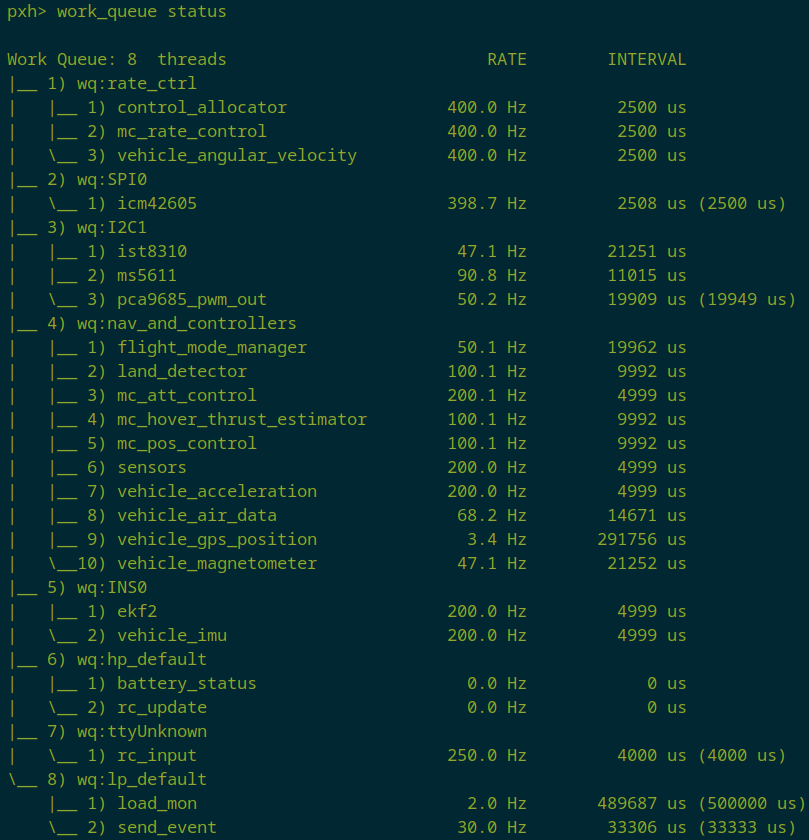
\includegraphics[width=1.0\textwidth]{./img/png/sspfs-px4-validation}
    \caption{PX4}%
    \label{fig:sspfs-app-validation-1}
  \end{subfigure}
  \begin{subfigure}[t]{0.49\textwidth}
    \centering
    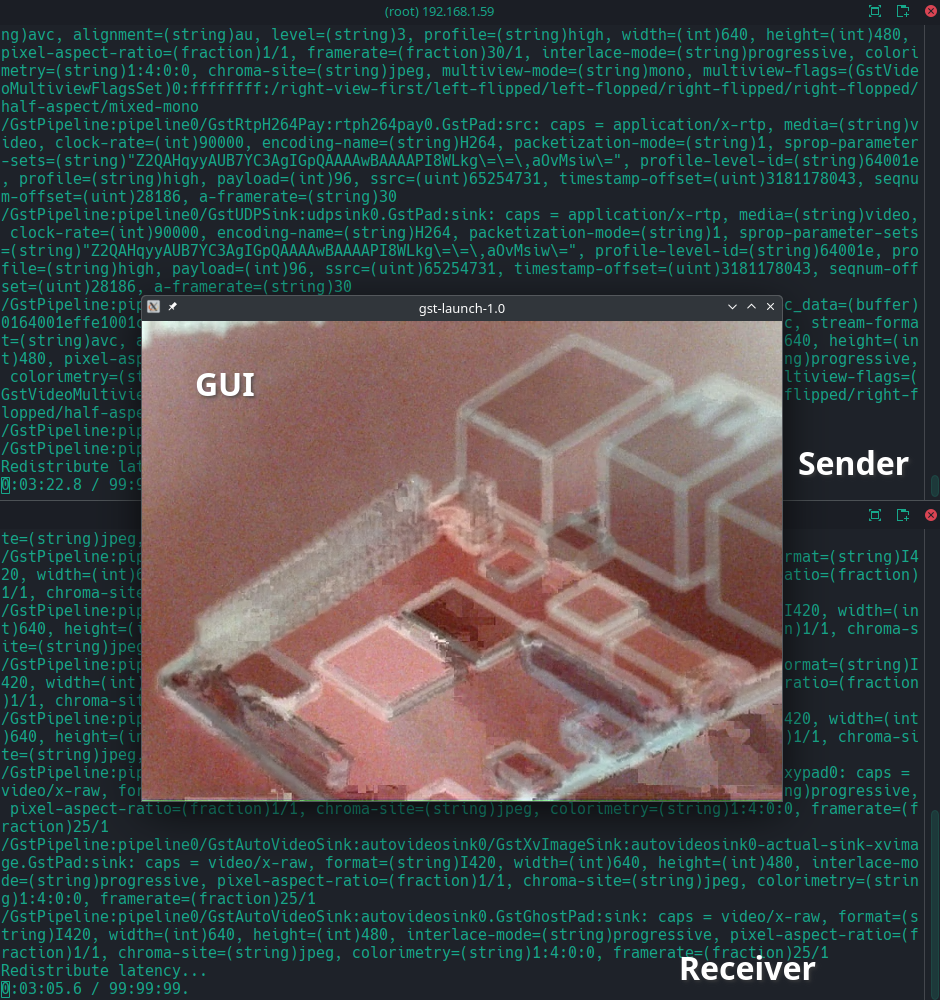
\includegraphics[width=\linewidth]{./img/png/sspfs-cam-qgc}
    \caption{Video surveillance}%
    \label{fig:sspfs-app-validation-2}
  \end{subfigure}
  \caption{SSPFS: validation of application software}
  \label{fig:sspfs-app-validation}
\end{figure}

\section{Functional tests}
\label{sec:functional-tests}
Fig.~\ref{fig:uav-main-eval-kmod} outlines the functional test methodology,
which assesses resilience under adversarial faults. We emulate compromises by
deploying a malicious user-space program (\lstinline{crash_app}) and a malicious
kernel module (\lstinline{crash_mod.ko}) against both \gls{uspfs} and
\gls{sspfs}.
%
In the unsupervised case, malicious components execute directly on the host
Linux \gls{os}; a process crash or kernel fault is expected to propagate
system-wide, terminating both the non-critical (video streaming) and
safety-critical (PX4) stacks, leading to loss of flight control.

In the supervised case, we deploy malicious components solely to the Companion
\gls{vm}, reflecting a likely compromise vector via Wi-Fi. Here, we expect the
hypervisor to contain the failure to the Companion \gls{vm}: a fatal user-space
abort or kernel fault triggers a guest crash while the PX4 \gls{vm} continues
operating, preserving flight capability.
%
This comparative setup demonstrates fault containment with \gls{sspfs}: critical
functions remain available despite failures in the non-critical domain.

\begin{figure}[!hbtp]
  \centering
  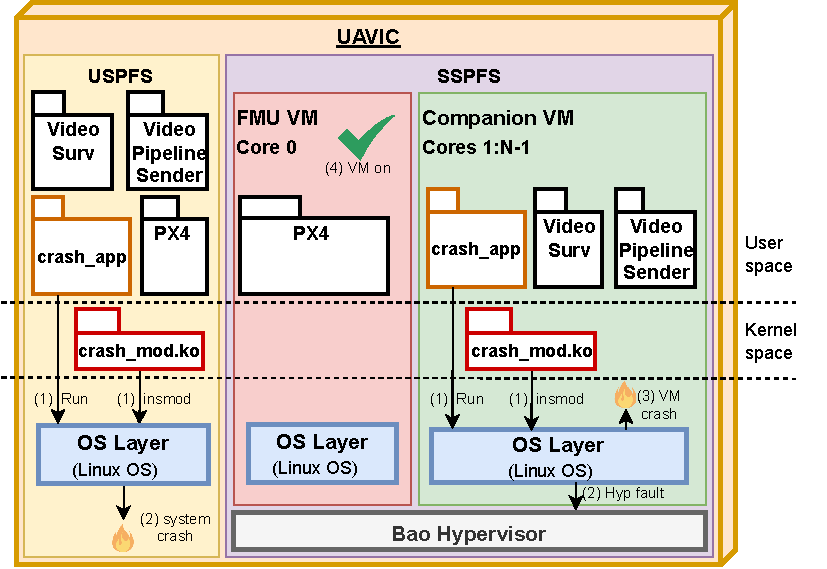
\includegraphics[width=0.8\textwidth]{./img/pdf/uav-main-eval-funcTest}
  \caption{Functional tests' overview}%
  \label{fig:uav-main-eval-kmod}
\end{figure}

\subsection{Privileged mode}
\label{sec:privileged-mode}
Malicious actors with privileged access -- via superuser escalation or corrupted
kernel modules -- pose severe risks. This section evaluates vulnerability to
privileged-mode attacks by deploying malicious kernel modules.
%
A basic kernel attack vector is an explicit \lstinline{panic} invocation, which
signals an unrecoverable state. Listing~\ref{lst:kmod-panic} (line 5) implements
this and shows the skeleton of a kernel module. Additional modules are in
\lstinline{eval/kmod/}~\cite{thesis-sw-github}. When executed, we expect: (1)
local interrupts and preemption disabled; (2) secondary cores halted; (3) a
\lstinline{Forced kernel panic!} message; (4) system reboot after a timeout or a
hang in an infinite loop.

\begin{longlisting}
\centering
\inputminted[]{c}{./listing/kmod_panic.c}
\caption[Functional tests: implementation of the panic kernel module]{Functional
  tests: implementation of the Panic kernel module (see
  \lstinline{panic_module.c}~\cite{thesis-sw-github})}
\label{lst:kmod-panic}
\end{longlisting}

Fig.~\ref{fig:kmod-panic-test-uspfs} shows testing on \gls{uspfs}. We boot via
\gls{uart} (1), then insert the malicious module over \gls{ssh} on Wi-Fi (2). The \gls{ssh}
session froze, and the host became unreachable (3), confirming a system-wide
crash (catastrophic \gls{uav} failure).

\begin{figure}[!hbt]
  \centering
  \begin{subfigure}[t]{0.8\textwidth}
    \centering
    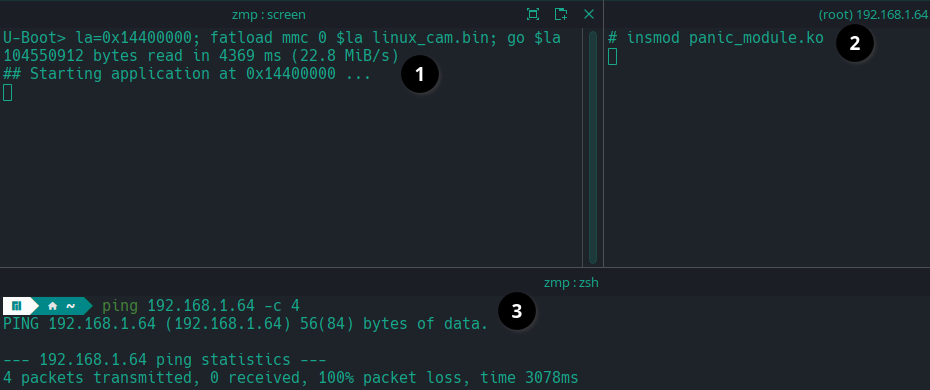
\includegraphics[width=1.0\textwidth]{./img/png/kmod-panic-test-annot}
    \caption{USPFS}%
    \label{fig:kmod-panic-test-uspfs}
  \end{subfigure}
  \begin{subfigure}[t]{0.8\textwidth}
    \centering
    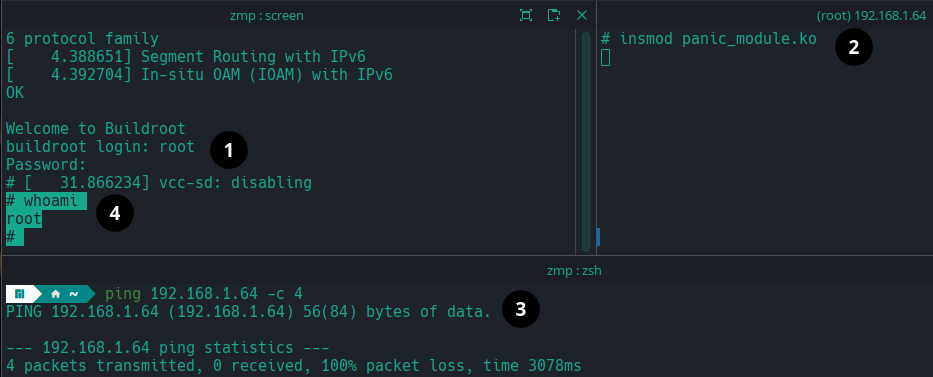
\includegraphics[width=\linewidth]{./img/png/kmod-panic-test-bao-annot}
    \caption{SSPFS}%
    \label{fig:kmod-panic-test-sspfs}
  \end{subfigure}
  \caption{Functional tests: panic kernel module testing}
  \label{fig:kmod-panic-test}
\end{figure}

We then repeated the test on \gls{sspfs}
(Fig.~\ref{fig:kmod-panic-test-sspfs}). The system was started from the U-Boot
\gls{uart} console, later used by Bao and the PX4 \gls{vm}, allowing login
(1). After inserting the malicious module via \gls{ssh} into the Companion \gls{vm}
(2), the \gls{ssh} session froze and the Companion \gls{vm} became unreachable
(3). The PX4 \gls{vm} continued running (4), preserving \gls{uav} control. These
results show that Bao maintains domain isolation under privileged-mode faults.

A memory corruption attack writes to an unmapped physical address using \lstinline{ioremap} of a valid but non-existent region (source in \lstinline{memcorrupt_module.c}~\cite{thesis-sw-github}). The write (line 36) is expected to fault due to missing physical backing~\cite{iomapLinux}. Results matched the panic case: \gls{uspfs} suffered a system-wide failure, whereas in \gls{sspfs} only the Companion \gls{vm} crashed and the PX4 \gls{vm} remained operational.

Memory exhaustion is induced by lowering the \gls{oom} score of the kernel
thread (line 11) to minimize kill likelihood, then allocating and pinning pages
in a loop (lines 15, 20) to prevent reclamation
(\lstinline{memhog_module.c}~\cite{thesis-sw-github}). Again, \gls{uspfs}
collapsed under pressure, while \gls{sspfs} contained the failure to the
Companion \gls{vm} and kept PX4 running.

Finally, terminating \lstinline{init} compromises the system. The module
(\lstinline{initkiller_module.c}~\cite{thesis-sw-github}) references
\lstinline{init} (line 16), walks its \glspl{vma} (line 28), pins pages (line
36), and corrupts the memory map (line 42), provoking failure. As before,
\gls{uspfs} crashed globally, whereas \gls{sspfs} preserved the PX4 \gls{vm} and
flight capability.

\clearpage

\subsection{Unprivileged mode}
\label{sec:unprivileged-mode}
User-space attacks expose a smaller surface because access to critical resources
is limited. A common tactic is to induce extreme contention that degrades
performance until the critical system becomes unresponsive, which can still lead
to a hazardous outcome in flight.
%
The user-space resource-exhaustion application is available at
\lstinline{eval/userspace/memhog_module.c}~\cite{thesis-sw-github}. It employs three concurrent vectors:
(1) memory exhaustion by unbounded allocation while attempting to evade the \gls{oom} killer (\lstinline{memory_attack()});
(2) process exhaustion via a fork storm that spawns processes which touch shared memory and then hang (\lstinline{process_attack()});
(3) \gls{cpu} and \gls{io} starvation (\lstinline{cpu_io_attack()}) by raising the process to the highest scheduling priority (line 132), issuing continuous random page reads (line 140), and forcing frequent rescheduling (line 143).

A monitoring thread (\lstinline{status_thread()}) records (1) elapsed time, (2) free memory via \lstinline{sysinfo()}, (3) process count \lstinline{sysinfo.procs}, (4) \gls{cpu} usage from \lstinline{/proc/stat}, and (5) load average from \lstinline{sysinfo.loads}. The \lstinline{main()} routine removes resource limits, launches the monitor, starts each attack in a child process, and then stays alive in a non-optimizable loop.

Fig.~\ref{fig:user-memhog-test-uspfs} shows testing on \gls{uspfs}. After boot over \gls{uart} (1) and SSH login over Wi-Fi (2), the system quickly became unresponsive (3). Basic commands such as \lstinline{ls} failed and resources were permanently pinned by the attack (4). Although the host still answered at the network level, it could no longer service PX4 or the video pipeline, severely impacting flight functionality.

We repeated the procedure on \gls{sspfs} (Fig.~\ref{fig:user-memhog-test-sspfs}). The platform was booted over \gls{uart}, bringing up the PX4 and Companion \glspl{vm}. After logging into the PX4 \gls{vm} (1), we connected to the Companion \gls{vm} via SSH (2) and started the attack there. The Companion \gls{vm} became unresponsive (3) and dedicated its resources to the attacker (4), but the PX4 \gls{vm} remained responsive and controllable. Hence only the non-critical domain failed, and the \gls{uav} retained flight capability.
%
These results confirm that Bao preserves critical-domain availability under severe user-space contention in the non-critical domain, meeting the consolidation and isolation goals.

\begin{figure}[!hbt]
  \centering
  \begin{subfigure}[t]{0.7\textwidth}
    \centering
    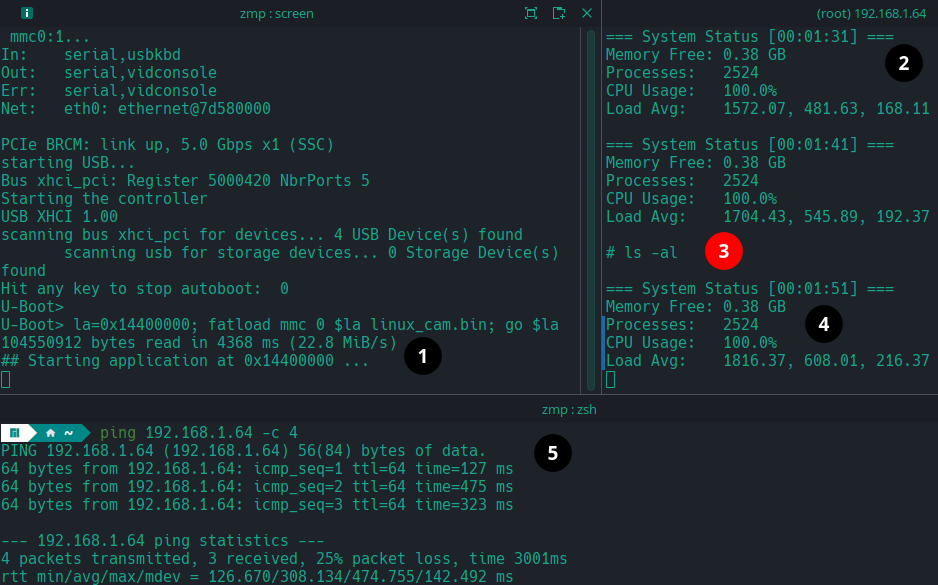
\includegraphics[width=1.0\textwidth]{./img/png/user-memhog-test-annot}
    \caption{USPFS}%
    \label{fig:user-memhog-test-uspfs}
  \end{subfigure}
  \begin{subfigure}[t]{0.7\textwidth}
    \centering
    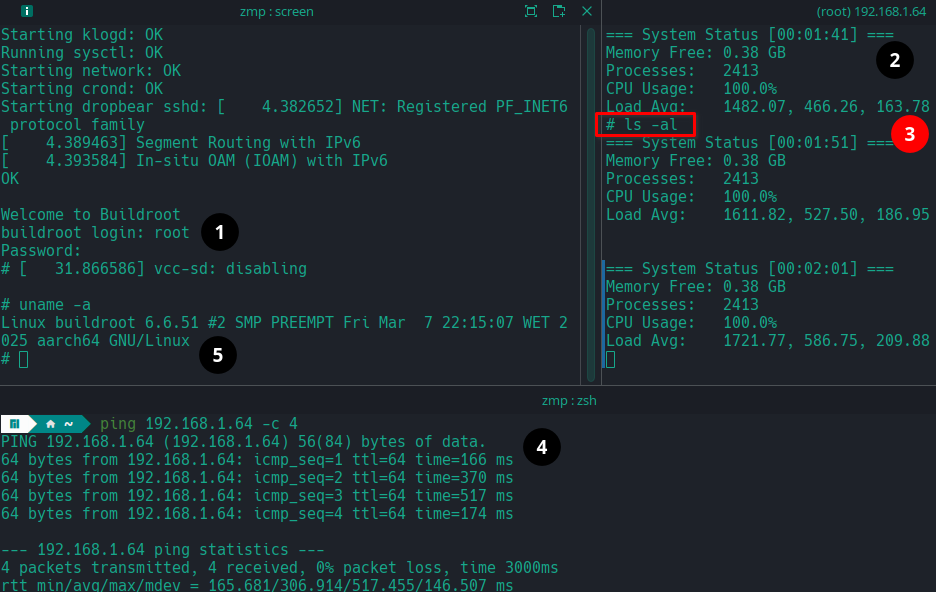
\includegraphics[width=\linewidth]{./img/png/user-memhog-test-bao-annot}
    \caption{SSPFS}%
    \label{fig:user-memhog-test-sspfs}
  \end{subfigure}
  \caption{Functional tests: user-space resource-exhaustion application}
  \label{fig:user-memhog-test}
\end{figure}

\section{Bao benchmarks}
\label{sec:bao-benchmarks}
Prior work has benchmarked the Bao hypervisor in mixed-criticality settings~\cite{martins2023shedding,costaIRQColoring2023}. We follow a similar methodology but focus strictly on performance. First, we establish a baseline on the \gls{uspfs} system (native execution). Then, we quantify the overhead introduced by Bao on the \gls{sspfs} system. Performance degradation (PD) is computed as the relative increase in execution time (ET):
\begin{equation}
  \label{eq:perform-deg}
  PD~(\%) \;=\;
  \frac{ET_{\text{SSPFS}} - ET_{\text{USPFS}}}{ET_{\text{USPFS}}}\cdot 100
\end{equation}

The test suite is MiBench \gls{aics}~\cite{guthaus2001mibench}, with both \emph{small} (resource-constrained) and \emph{large} (realistic load) variants. On Linux guests we use \lstinline{perf}~\cite{perfLinux} to time executions and collect microarchitectural counters; bare-metal guests use the Arm Generic Timer (10~ns resolution) with a custom \gls{pmu} driver. The monitored events include: (1) instruction count; (2) \gls{tlb} accesses/refills; (3) cache accesses/refills; (4) exceptions; and (5) interrupts.
%
To study inter-VM interference, we deploy a custom bare-metal guest with three
\glspl{vcpu} that continuously stream writes into a buffer sized to the
\gls{llc}, creating a sustained memory subsystem load (not necessarily
worst-case, but intentionally heavy).

Fig.~\ref{fig:uav-main-eval-mibench} summarizes the workflow: build guests (Linux+\lstinline{perf} for MiBench and the interference guest), run experiments, capture logs, and plot results~\cite{shedlightRepo}. We evaluate the \gls{uspfs} baseline and four \gls{sspfs} configurations:
\lstinline{mibench} (Linux guest on Bao),
\lstinline{mibench+col} (+ page coloring),
\lstinline{mibench+interf} (+ interference guest),
and \lstinline{mibench+interf+col} (+ interference and coloring).
For each run we place the executable \lstinline{BIN} (\lstinline{linux.bin} or
\lstinline{bao.bin}) on the SD card (1), open a persistent capture from
\gls{gcs} to \gls{uavic} (2), power on (3), start the binary from U-Boot (4),
and append results to a log file (8). Some test runs require a second binary
\lstinline{BIN2} (e.g., iterating the full MiBench set) whose output is
redirected into the same log (7). We then close the log and plot relevand data
with a Python script. All MiBench configuration files, logs, and plotting scripts are in
\lstinline{mibench/}~\cite{thesis-sw-github}.

\begin{figure}[!hbt]
  \centering
  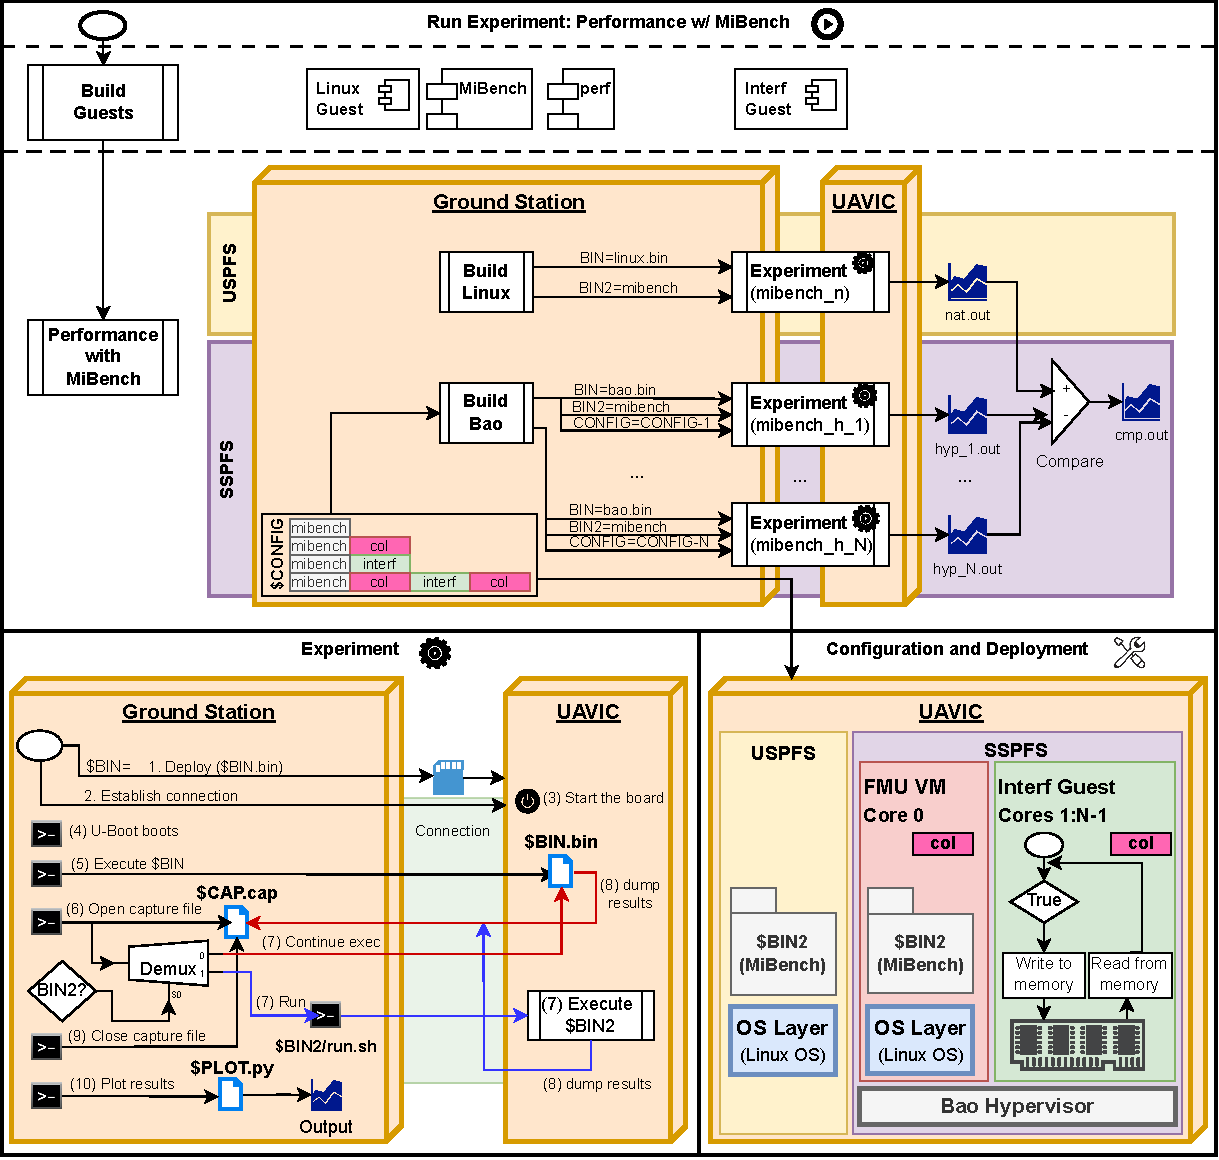
\includegraphics[width=1.0\textwidth]{./img/pdf/uav-main-eval-mibench}
  \caption{Bao performance benchmarking workflow}%
  \label{fig:uav-main-eval-mibench}
\end{figure}

Fig.~\ref{fig:plot-performDeg-Base} reports relative PD for MiBench \gls{aics} across three configurations:
(1) \hlighthex{0097FF}{000000}{\textbf{baremetal-noMail}} — native execution without the mailbox driver patch;
(2) \hlighthex{399334}{000000}{\textbf{bao-noMail}} — Linux guest on Bao without the mailbox driver patch; and
(3) \hlighthex{FF9E00}{000000}{\textbf{bao}} — Linux guest on Bao with the mailbox driver patch.
Average baseline execution times are printed below each benchmark. PD is small
overall, especially for longer-running benchmarks (suffix \lstinline{large},
e.g., \lstinline{basicmath large}, \lstinline{qsort large}). The mailbox patch
adds negligible overhead and Bao's contribution to PD is also modest.

\begin{figure}[!hbt]
  \centering
  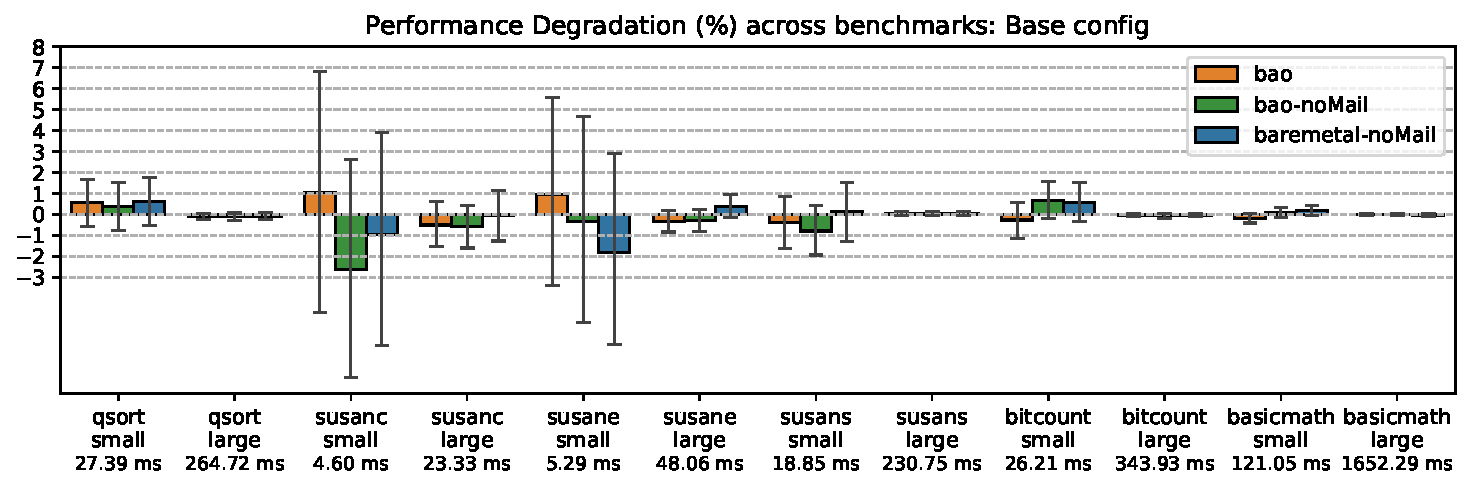
\includegraphics[width=1.0\textwidth]{./img/pdf/plot-performDeg-Base}
  \caption{Relative performance degradation (\%) for MiBench AICS}%
  \label{fig:plot-performDeg-Base}
\end{figure}

Fig.~\ref{fig:plot-performDeg-Interf} shows PD under cache partitioning and interference for:
(1) \hlighthex{FF9E00}{000000}{\textbf{bao+col}} — MiBench on VM1 with two cache colors;
(2) \hlighthex{399334}{000000}{\textbf{bao+interf}} — MiBench on VM1 with the interference guest on VM2 using three \glspl{cpu}; and
(3) \hlighthex{0097FF}{000000}{\textbf{bao+interf+col}} — MiBench on VM1 with two colors, plus the interference guest on VM2 using three \glspl{cpu} and two colors.
Colors are evenly split between VMs; average baseline times appear below each benchmark. Interference significantly raises PD, especially for short runs (suffix \lstinline{small}, e.g., \lstinline{susanc small}, \lstinline{susane small}), while longer runs are less sensitive. Page coloring consistently mitigates interference for VM1, reducing PD across the set.

\begin{figure}[!hbt]
  \centering
  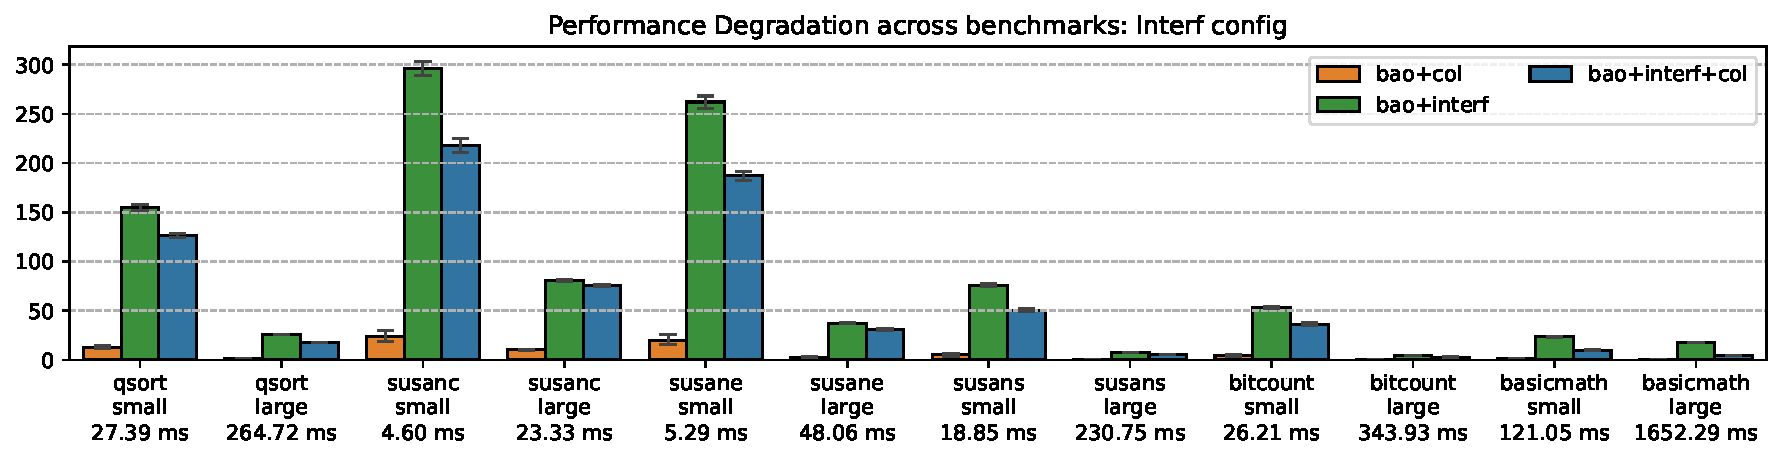
\includegraphics[width=1.0\textwidth]{./img/pdf/plot-performDeg-Interf}
  \caption{Relative performance degradation (\%) for MiBench AICS under cache partitioning and interference}%
  \label{fig:plot-performDeg-Interf}
\end{figure}

\subsection{Guests benchmarking}
\label{sec:guests-benchmarking}
We benchmark each \gls{vm} separately with application-specific metrics, then compare \gls{uspfs} and \gls{sspfs} using those metrics.

\subsubsection{FMU VM}
\label{sec:fmu-vm}
The \gls{fmu} \gls{vm} runs PX4 atop Linux under the Bao hypervisor. We adapted
the MiBench-based methodology to profile PX4 with \lstinline{perf}. Unlike
MiBench (finite runs), PX4 is long-running, so we use \lstinline{perf --timeout}
to fork PX4, collect counters for a fixed interval, and terminate the child.

Listing~\ref{lst:perf-px4} shows the procedure: five warm-up runs and twenty
30 seconds test runs. The \lstinline{px4_bench()} helper invokes \lstinline{perf}
with the desired events/timeout and the PX4 launch command (lines 6--17). We
then set the events (line 18) and call \lstinline{px4_bench} for warm-up and
measured runs.

\begin{longlisting}
\centering
\inputminted[]{bash}{./listing/perfPX4.sh}
\caption{PX4 benchmarking using \texttt{perf}}
\label{lst:perf-px4}
\end{longlisting}

Wall-clock time is unsuitable here (forced termination dominates): native
averaged $30.044213 \pm 0.000613$\,s and Bao $30.04608 \pm 0.00199$\,s (max PD
$\approx 0.015\%$). Instead, we compute PD from the instruction count
(\lstinline{r08:uk}). Native recorded $3{,}077{,}590{,}067$ events versus Bao’s
$3{,}016{,}875{,}258$, a small degradation of $1.97\%$.

For critical systems, deadline compliance matters most. PX4 supports (i)
traditional tasks (dedicated stacks/priorities) and (ii) work-queue tasks
(shared stacks/priorities), the latter preferred for
efficiency~\cite{px4WorkQueue}. We therefore profile work-queue update rates for
six critical
operations~\cite{px4ModulesRefCtrl,px4ModulesRefDriver,px4ModulesRefSystem}:
(1) \lstinline{control_allocator} (torque/thrust to actuator setpoints);
(2) \lstinline{mc_rate_control} (multicopter rate control);
(3) \lstinline{pca9685_pwm_out} (\gls{i2c} PWM to \gls{esc} motors);
(4) \lstinline{flight_mode_manager} (setpoint generation per flight mode);
(5) \lstinline{mc_pos_control} (position/velocity control);
(6) \lstinline{sensors} (acquisition/publish).

To query PX4 while running, we inject \lstinline{work_queue status} via a shared
\gls{fifo}. The script \lstinline{px4_wq_run.sh} (see~\cite{thesis-sw-github})
creates the FIFO (line 12), launches PX4 and captures its PID (lines 13--15),
writes periodic commands (lines 28--32), then shuts down and cleans up. We run
five warm-ups followed by twenty measured runs under both native and Bao. Each
run issues \lstinline{work_queue status} every 10\,s for 3\,min (18
samples/run).

Fig.~\ref{fig:px4-sched-overhead} reports results. The x-axis lists the tasks
and the native mean update interval (\textmu s) as the baseline. Bars show Bao’s
mean scheduling overhead and standard deviation, defined as:

\begin{equation}
  \label{eq:1}
  \mu_{ov} (\%) = \frac{\mu_{bao} - \mu_{bm}}{\mu_{bm}} \cdot 100
\end{equation}
\begin{equation}
  \label{eq:2}
  \sigma_{ov} (\%) = \sqrt{ \left(\frac{\sigma_{bao}}{\mu_{bao}}\right)^{2} +
    \left(\frac{\sigma_{bm}}{\mu_{bm}}\right)^{2} } \cdot 100
\end{equation}

\begin{figure}[!hbt]
  \centering
  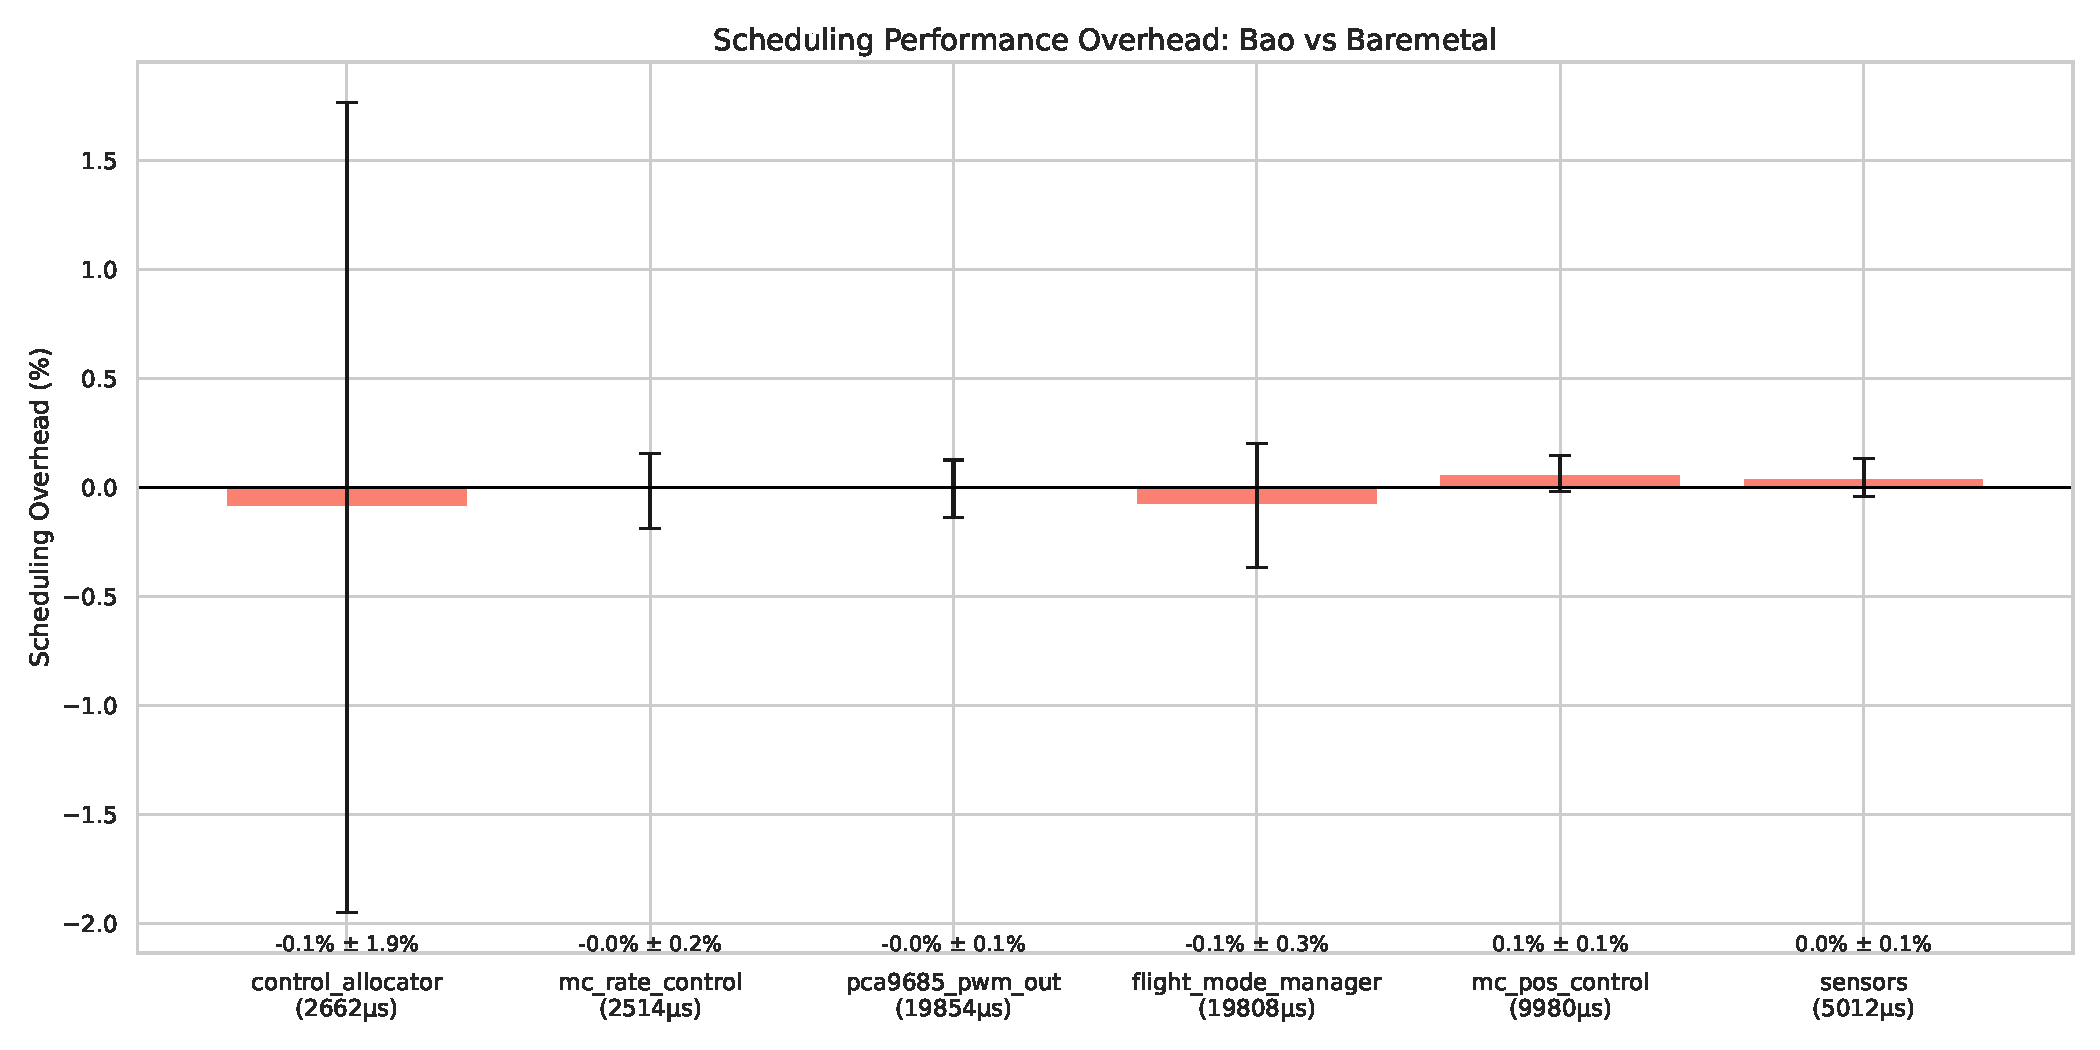
\includegraphics[width=1.0\textwidth]{./img/pdf/px4-sched-overhead} 
  \caption{PX4 tasks scheduling overhead}%
  \label{fig:px4-sched-overhead}
\end{figure}

Overheads are very low across tasks. Notably, \lstinline{pca9685_pwm_out} (motor
actuation) shows negligible overhead, while \lstinline{control_allocator}
(control-loop core) remains $\leq 2\%$. Overall, consolidating PX4 with Bao
imposes minimal scheduling overhead on the critical \gls{fmu}.

\subsubsection{Companion VM}
\label{sec:companion-vm}
The Companion \gls{vm} runs the \lstinline{gstreamer} pipeline for video capture
and streaming to the \gls{gcs}. User experience is driven primarily by two
metrics: sender-side \gls{fps} and end-to-end frame latency
(capture-to-reception delay). These can be distorted by external factors (e.g.,
\gls{gcs} \gls{cpu} load or network jitter).
%
To isolate consolidation overheads from environmental noise, we measure frame
rate on the \gls{uav} side. The script \lstinline{cam_fps.sh}
(see~\cite{thesis-sw-github}) runs the pipeline locally and reports
\gls{fps}. We execute five warm-up runs and twenty 2-minute test runs, then
terminate the pipeline.
%
Fig.~\ref{fig:fps-cmp} reports the relative \gls{fps} performance degradation
(Bao versus native) across runs, computed with Equation~\ref{eq:1} and
Equation~\ref{eq:2}. Most runs are near 0\% degradation; the worst case stays
below 2\%. Confidence intervals are narrow and include 0\%, indicating no
statistically significant \gls{fps} penalty from Bao.

\begin{figure}[!hbt]
  \centering
  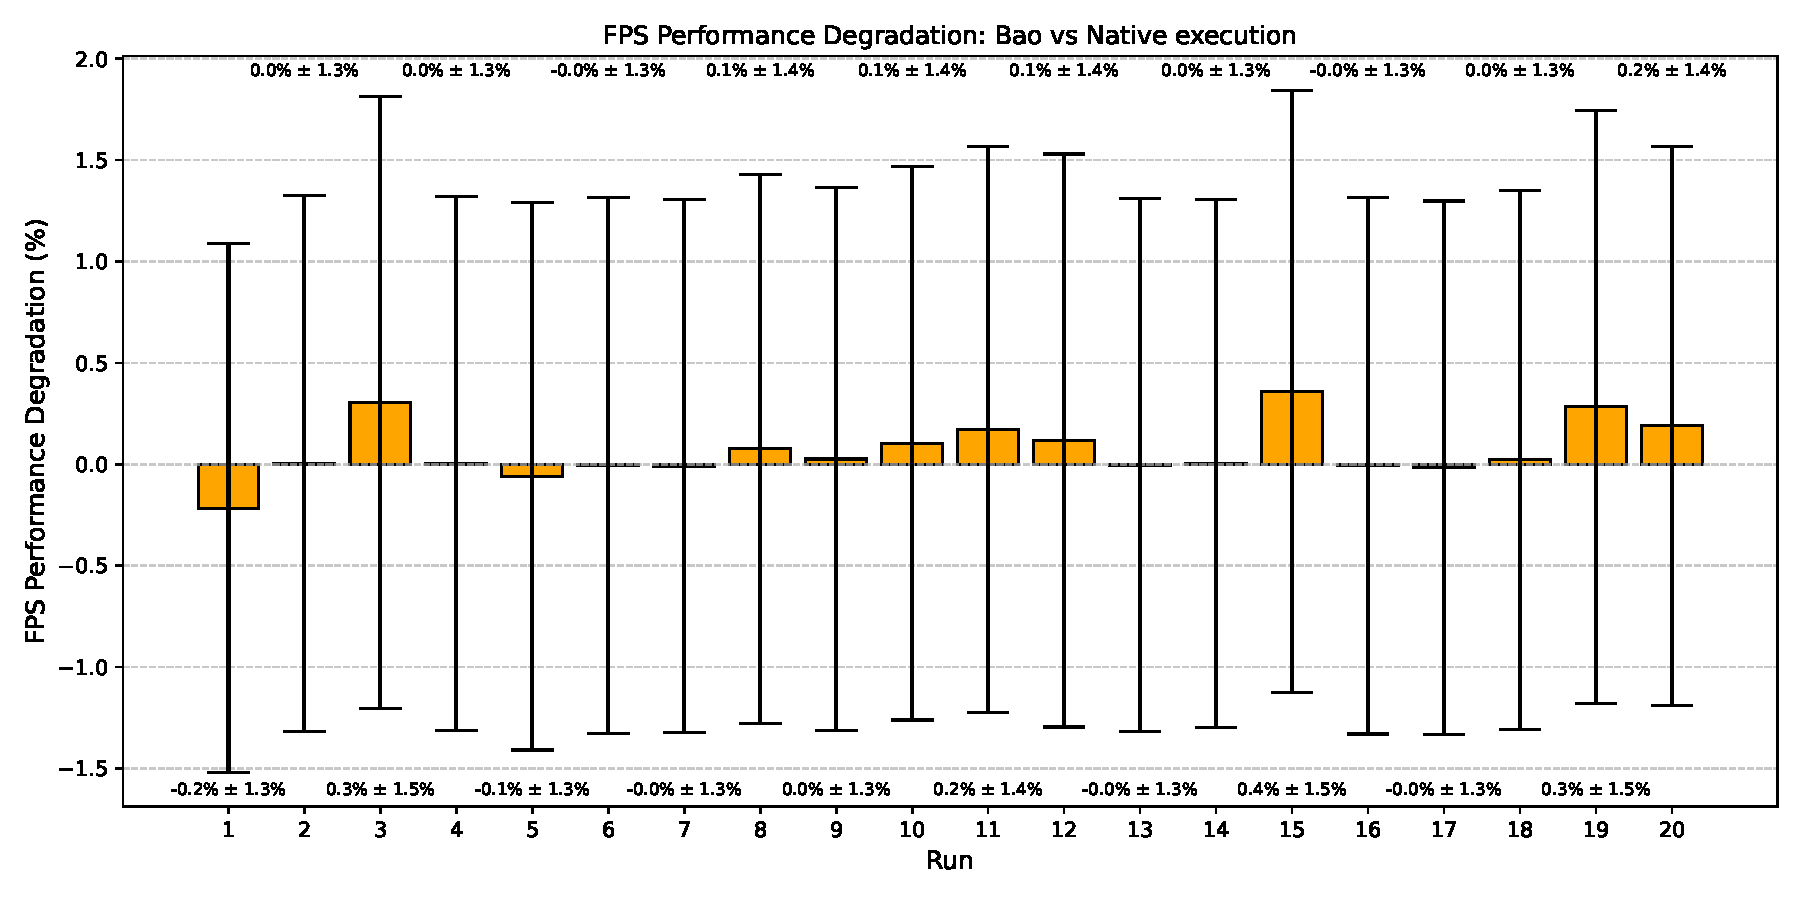
\includegraphics[width=1.0\textwidth]{./img/pdf/fps-cmp} 
  \caption{Relative FPS performance degradation: Bao versus native execution}%
  \label{fig:fps-cmp}
\end{figure}

\subsection{USPFS vs SSPFS}
\label{sec:uspfs-vs-sspfs}
After benchmarking guests individually, we compare \gls{uspfs} and \gls{sspfs} by running PX4 scheduling measurements and camera \gls{fps} tests concurrently on each system, logging data per-architecture.

Fig.~\ref{fig:px4-sspfs-uspfs} contrasts scheduling overheads and shows the
effect of cache coloring. The baseline is \gls{uspfs}; orange and blue bars
denote \gls{sspfs} with and without coloring, respectively. Positive values
indicate degradation; negative values indicate improvement. \gls{sspfs} shows
only marginal degradation (~1\%) for \lstinline{flight_mode_manager} and
\lstinline{pca9685_pwm_out}, while outperforming \gls{uspfs} elsewhere -- most
notably \lstinline{control_allocator} (6–15\% improvement).

\begin{figure}[!hbt]
  \centering
  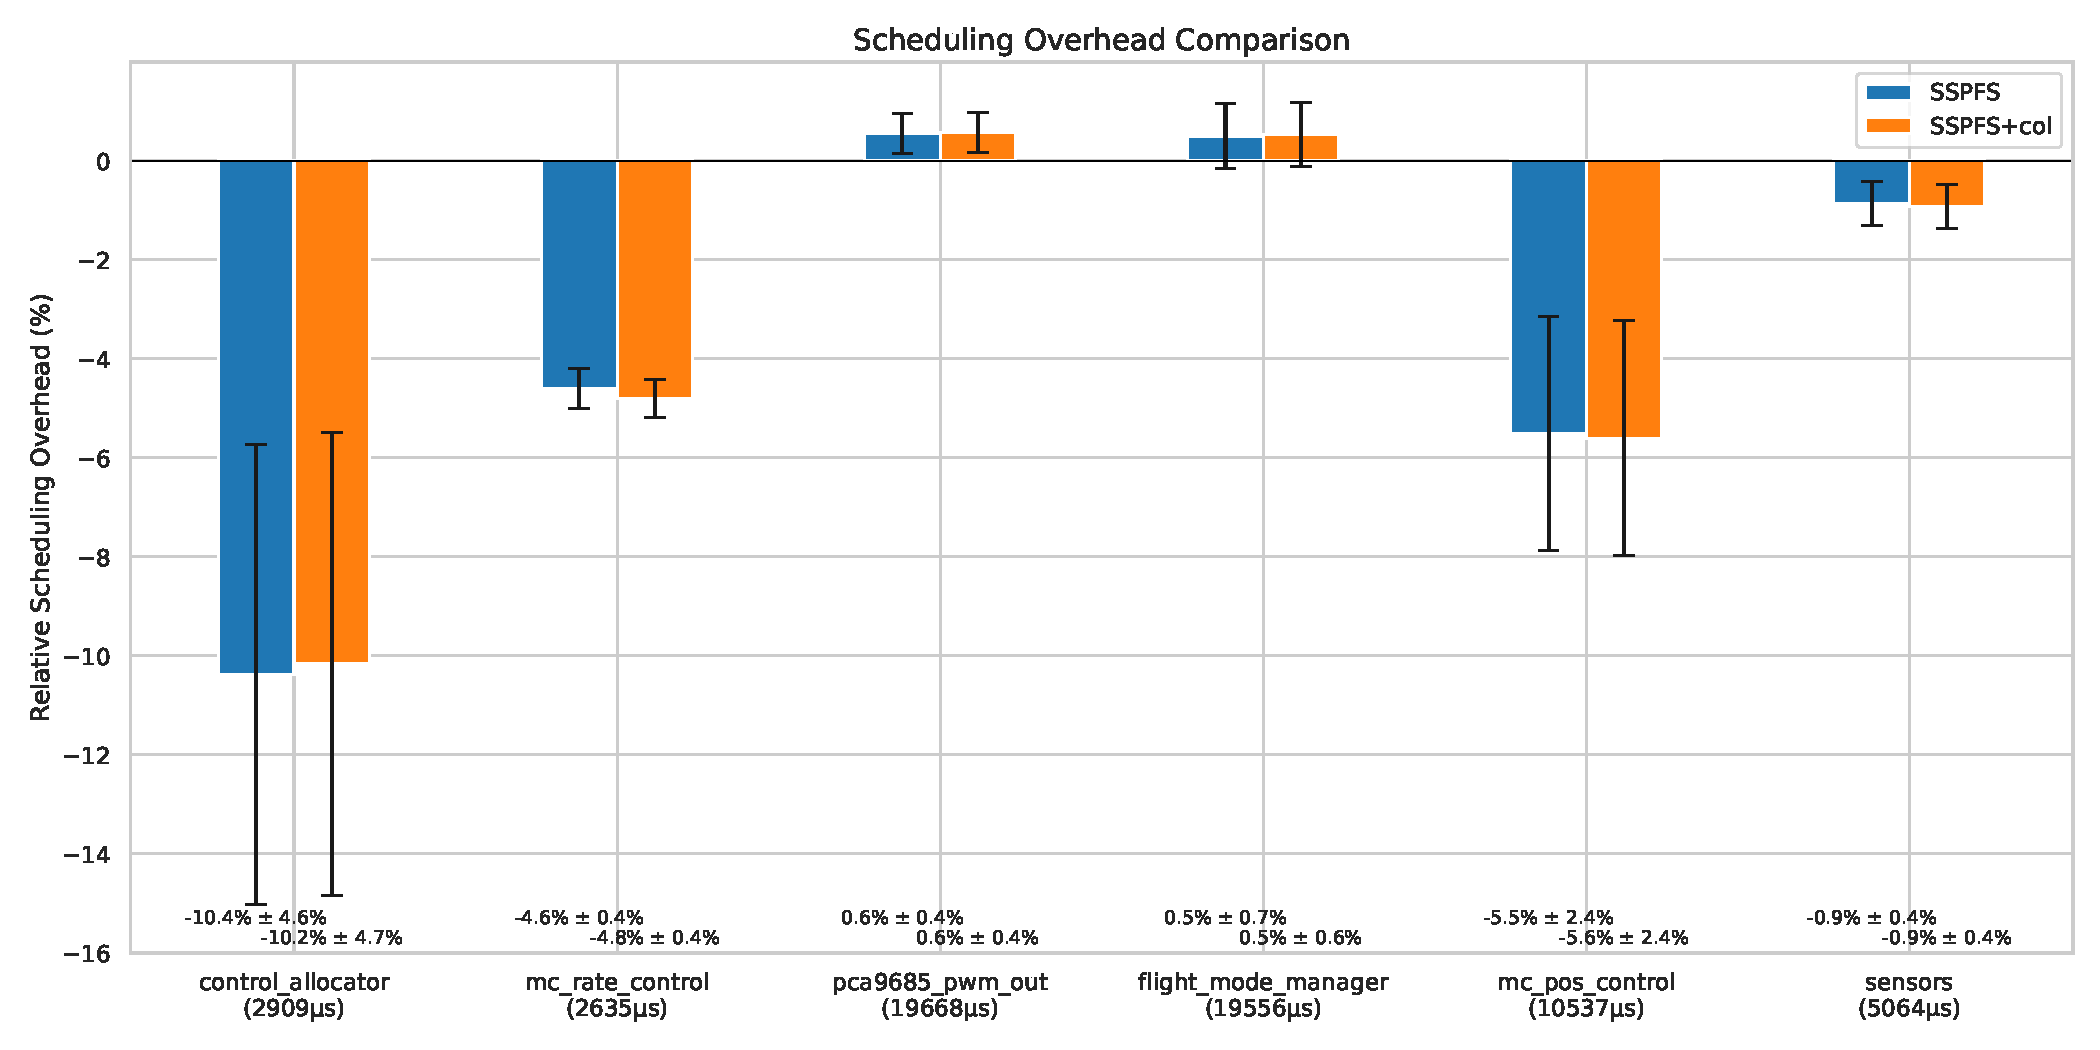
\includegraphics[width=1.0\textwidth]{./img/pdf/px4-sspfs-uspfs} 
  \caption{PX4 task scheduling overhead: USPFS versus SSPFS}%
  \label{fig:px4-sspfs-uspfs}
\end{figure}

We attribute this divergence to Bao’s isolation: \gls{uspfs} processes contend
for shared resources, whereas \gls{sspfs} \glspl{vm} enjoy statically
partitioned resources. Cache coloring yields only marginal gains on the
\gls{uavic} due to \gls{dma} constraints from \gls{spi} sensors; required
\gls{dma} mappings in the first 1\,GiB constrain virtual-coloring
effectiveness. Listing~\ref{lst:place-phys} shows the enforced physical
placement in the \gls{sspfs} configuration via \lstinline[keepspaces=true]|place_phys = true|.

\begin{longlisting}
\centering
\inputminted[]{bash}{./listing/placePhys.c}
\caption[Physical memory mapping in the SSPFS system]{Physical memory mapping in \gls{sspfs}: \lstinline[keepspaces=true]|place_phys = true|}
\label{lst:place-phys}
\end{longlisting}

Fig.~\ref{fig:cam-sspfs-uspfs} compares relative \gls{fps} degradation across
systems and evaluates cache coloring. Most runs show no statistically
significant difference (whiskers include 0). Runs 10 and 20 exhibit notable
outliers with over 30\% improvement, while coloring again has limited impact
given \gls{dma} constraints. These results align with the Companion \gls{vm}
microbenchmarks, indicating minimal impact on video performance.

\begin{figure}[!hbt]
  \centering
  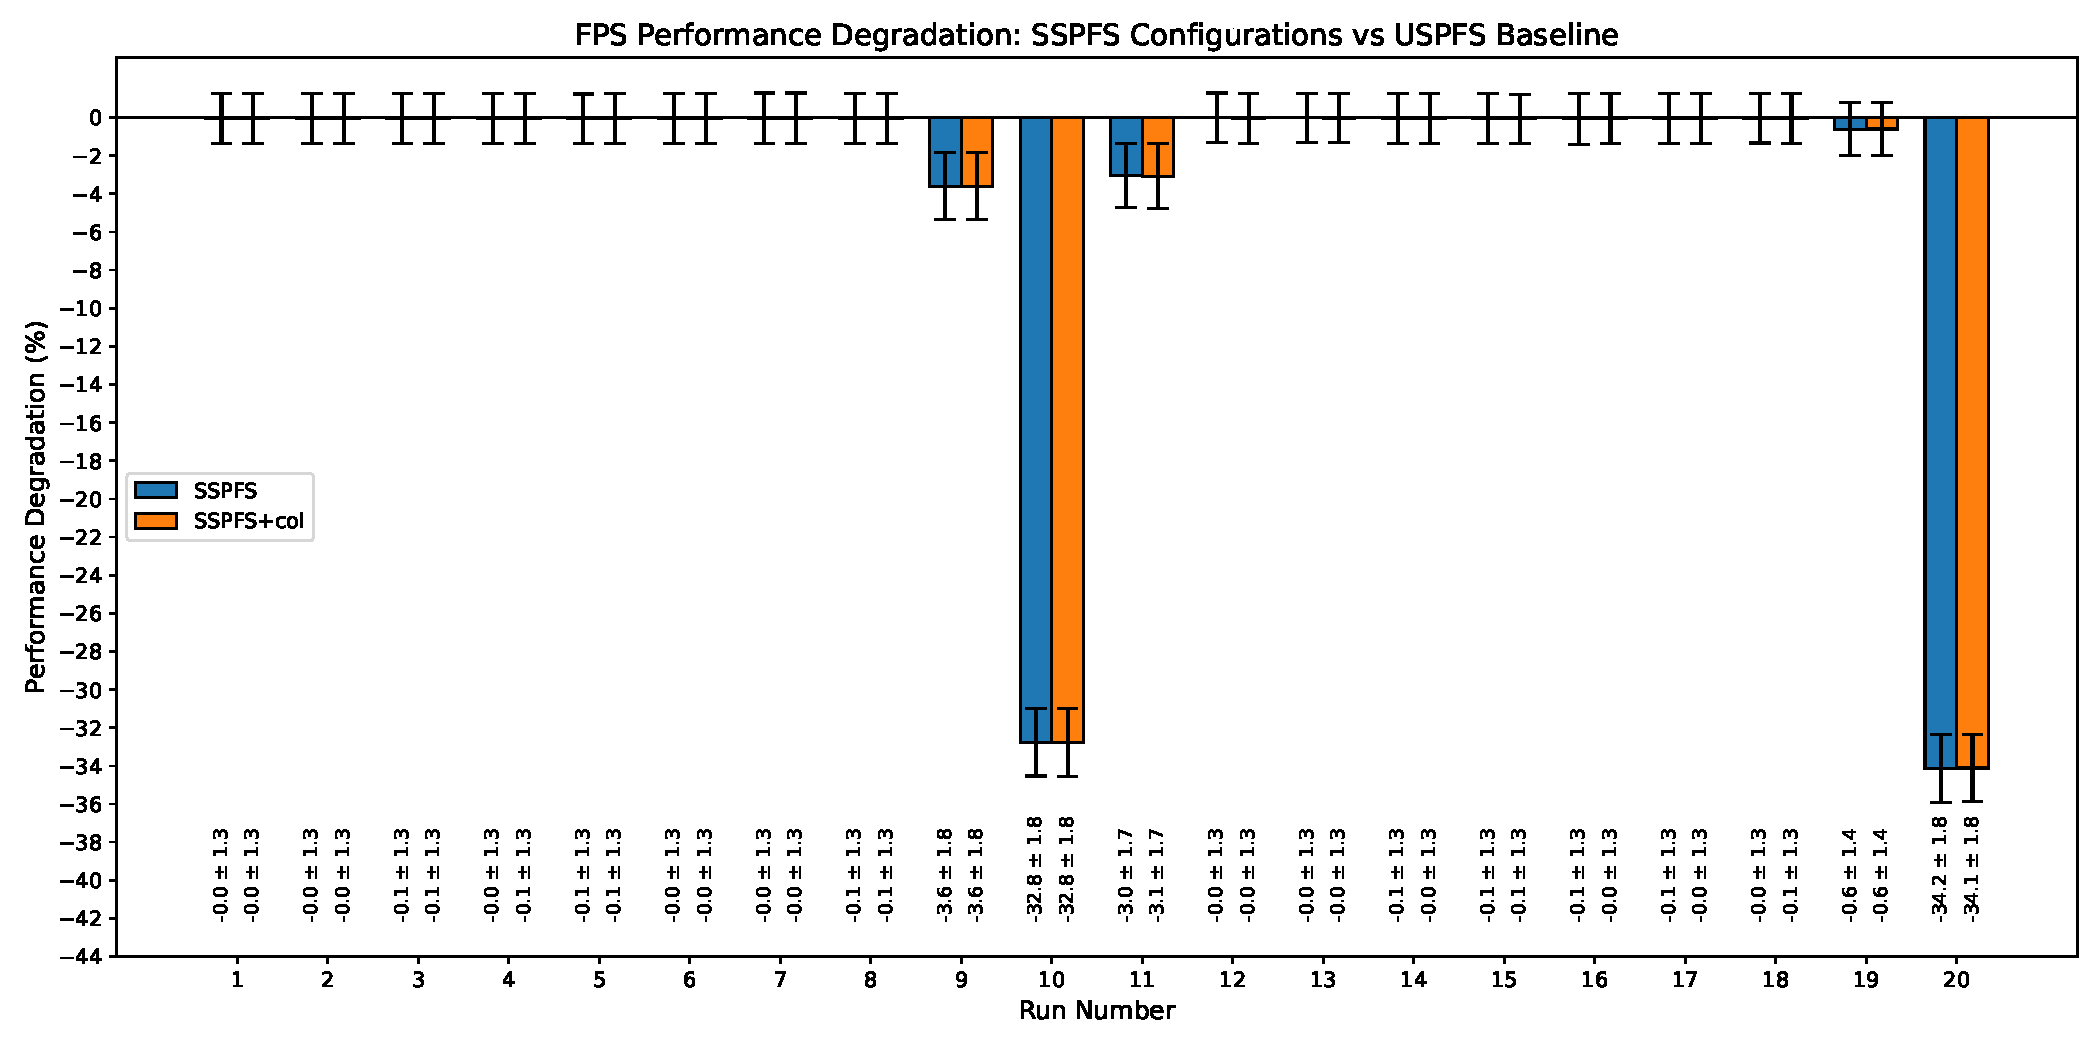
\includegraphics[width=1.0\textwidth]{./img/pdf/cam-sspfs-uspfs} 
  \caption{Relative FPS performance degradation: USPFS versus SSPFS}%
  \label{fig:cam-sspfs-uspfs}
\end{figure}

Overall, beyond isolation benefits, \gls{sspfs} can deliver performance
advantages in mixed-criticality consolidation. Static resource partitioning
reduces contention seen in \gls{uspfs}, making \gls{sspfs} a strong choice for
integrating flight control and video surveillance.

\section{UAV benchmarks}
\label{sec:uav-benchmarks}
Finally, we evaluated both flight stacks under realistic conditions.
To this end, we configured an automated mission in QGroundControl
(Fig.~\ref{fig:mission-final}), ensuring a repeatable flight profile that can be used
to benchmark the \gls{uspfs} and \gls{sspfs} systems in real-flight scenarios.
%
The mission design incorporates two critical geospatial elements. An
external polygon defines the geofence perimeter, which triggers a
return-to-home failsafe if violated. The internal path is the flight path from
takeoff \lstinline{T} to landing \lstinline{L}. At takeoff, the \gls{uav} ascends
to an altitude of two meters and flies to waypoint \lstinline{3}, then reverses
direction and proceeds to \lstinline{4}, concluding at \lstinline{L} while maintaining a constant altitude. During landing, the \gls{uav} reduces speed to enable a safe, smooth touchdown.

\begin{figure}[!hbt]
  \centering
  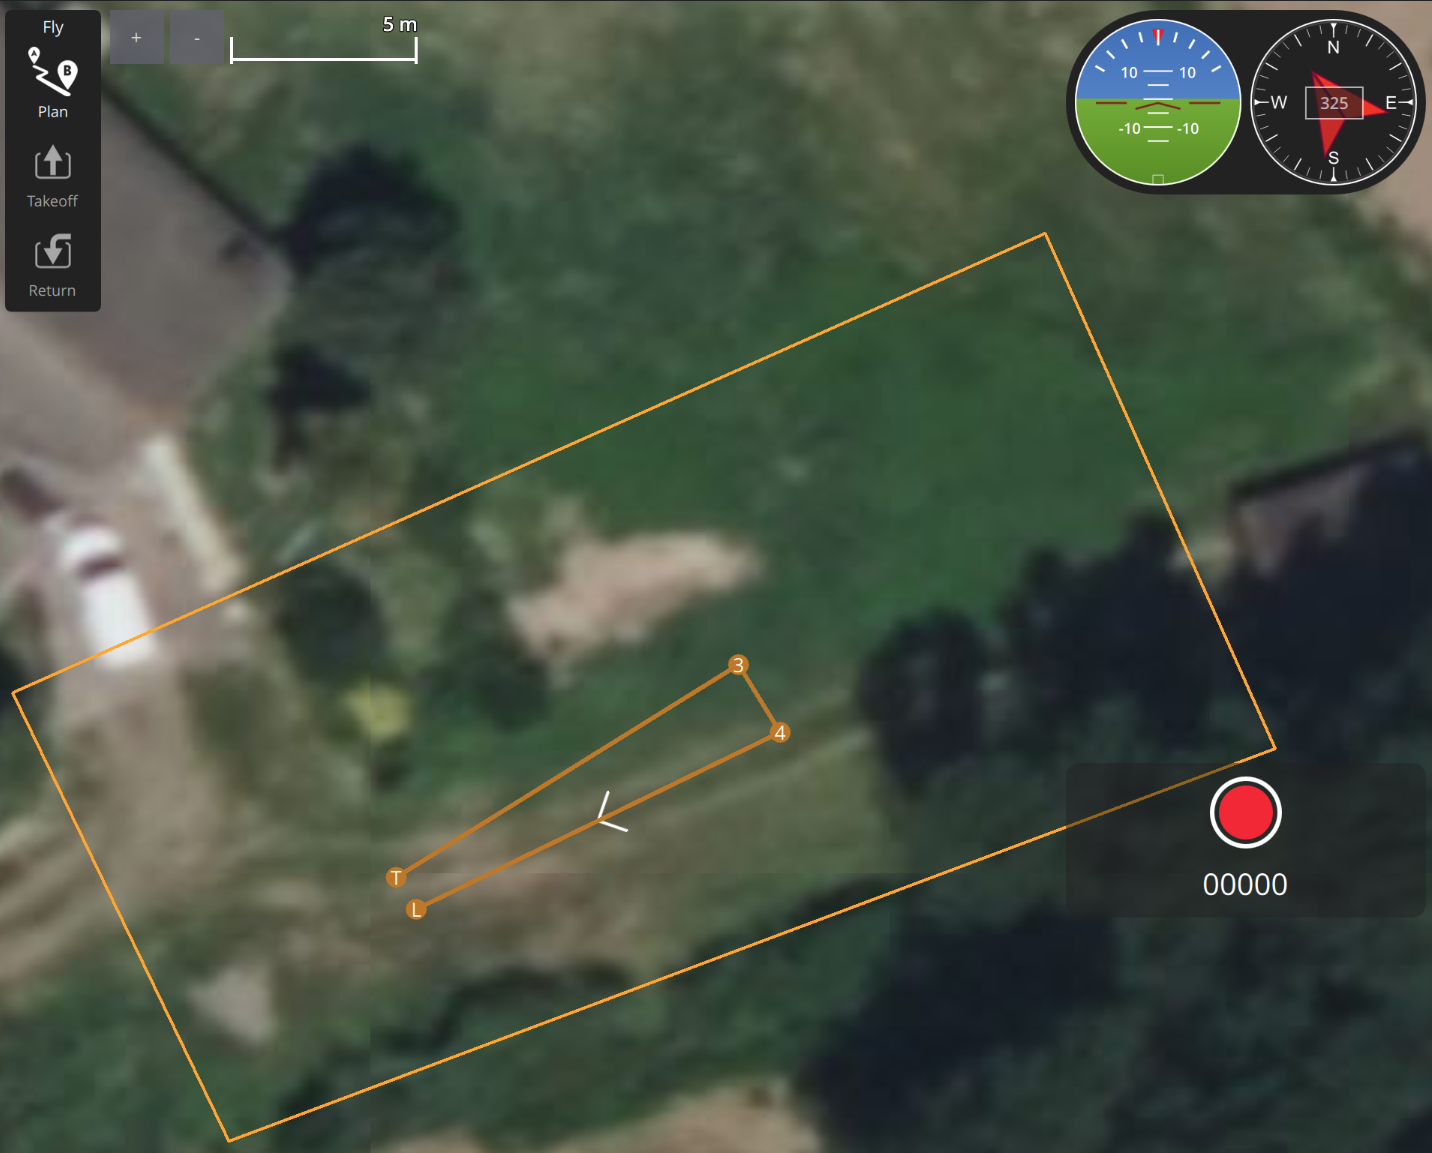
\includegraphics[width=0.7\textwidth]{./img/png/mission-final} 
  \caption{Automated mission configuration in QGroundControl}%
  \label{fig:mission-final}
\end{figure}

We performed a total of 33 flights per system under consistent
weather conditions. Each system was tested in a batch, as switching
between systems requires significant battery and time resources, preventing
randomized sequencing.
The flight logs were preserved for subsequent analysis of two critical metrics:
(1) position-tracking accuracy and (2) system resource utilization patterns.
The sample size was chosen to achieve statistical power sufficient to detect meaningful
differences in these operational parameters.
%
PX4 flight logs are stored as ULog files (\lstinline{.ulg}), containing
\gls{uorb} topic messages subscribed to or published by various
modules. Specifically, we analyzed the \lstinline{vehicle_local} and
\lstinline{vehicle_local_setpoint} topics for position-tracking assessment, and
the \lstinline{cpuload} topic to evaluate system resource
utilization.
%
To account for temporal variations between flights, the time domain was
normalized to a mission-progress scale $[0, 100]$ using linear interpolation:
\begin{equation}
t_{\text{norm}} = \frac{t - t_{\min}}{t_{\max} - t_{\min}} \cdot 100
\end{equation}
where $t$ is the original timestamp, and $t_{\min}$ and $t_{\max}$ represent the start and end times of each flight, respectively.
%
At each normalized time point $\tau$, the 95\% confidence intervals for group
means were calculated using the Student's $t$-distribution~\cite{t-test}:
\begin{equation}
\text{CI}(\tau) = \bar{x}(\tau) \pm t_{\alpha/2, df} \cdot \frac{s(\tau)}{\sqrt{n(\tau)}}
\end{equation}
where:
\begin{itemize}
    \item $\bar{x}(\tau)$ is the sample mean at progress $\tau$,
    \item $s(\tau)$ is the sample standard deviation,
    \item $n(\tau)$ is the number of valid observations,
    \item $df = n(\tau) - 1$ degrees of freedom,
    \item $t_{\alpha/2, df}$ is the critical $t$-value ($\alpha = 0.05$).
\end{itemize}

Statistical significance between systems was evaluated using the two-sided
Welch unequal-variance $t$-test at each mission-progress point. This method is
preferred over the pooled-variance $t$-test, as the samples are independent and variances may differ~\cite{welch-t-test}:
\begin{equation}
  \label{eq:welch-t-test}
t(\tau) = \frac{\bar{x}_1(\tau) - \bar{x}_2(\tau)}{\sqrt{\frac{s_1^2(\tau)}{n_1(\tau)} + \frac{s_2^2(\tau)}{n_2(\tau)}}}
\end{equation}
%
The degrees of freedom were computed via:
\begin{equation}
  \label{eq:welch-t-test-df}
df(\tau) = \frac{\left( \frac{s_1^2(\tau)}{n_1(\tau)} + \frac{s_2^2(\tau)}{n_2(\tau)} \right)^2}{\frac{s_1^4(\tau)}{n_1^2(\tau)\,(n_1(\tau)-1)} + \frac{s_2^4(\tau)}{n_2^2(\tau)\,(n_2(\tau)-1)}}
\end{equation}

The null hypothesis ($H_0$) states no statistical difference between systems:
\begin{equation}
H_0: \mu_{\text{\gls{uspfs}}}(\tau) = \mu_{\text{\gls{sspfs}}}(\tau)
\end{equation}
$H_0$ was rejected at the $\alpha = 0.05$ significance level when $p(\tau) <
0.05$. The \lstinline{cmpLogs.py} Python script (see~\cite{thesis-sw-github})
contains implementation details for the log analysis.
% with false discovery rate controlled pointwise across the mission timeline.

Fig.~\ref{fig:mission-exec-sspfs} illustrates key phases of a mission
executing on the \gls{sspfs} system, while
Fig.~\ref{fig:mission-final-actual} shows the actual flight path.
Fig.~\ref{fig:mission-exec-case1} depicts the takeoff stage alongside the
software components used, including: (1) QGroundControl for mission flight
management and logging on the host system (2); (3) the \lstinline{gstreamer}
receiver pipeline with its \gls{gui} executing on the host (6); the
U-Boot loader and the \gls{fmu} \gls{vm} console responsible for PX4 execution
(4); and the \lstinline{gstreamer} sender pipeline running on the Companion
\gls{vm}, accessed via a remote \gls{ssh} connection over Wi-Fi.

% Figure environment with subfigures
\begin{figure}[!hbt]
  \centering
  % Row 1: Full width
  \begin{subfigure}[t]{\textwidth}
    \centering
    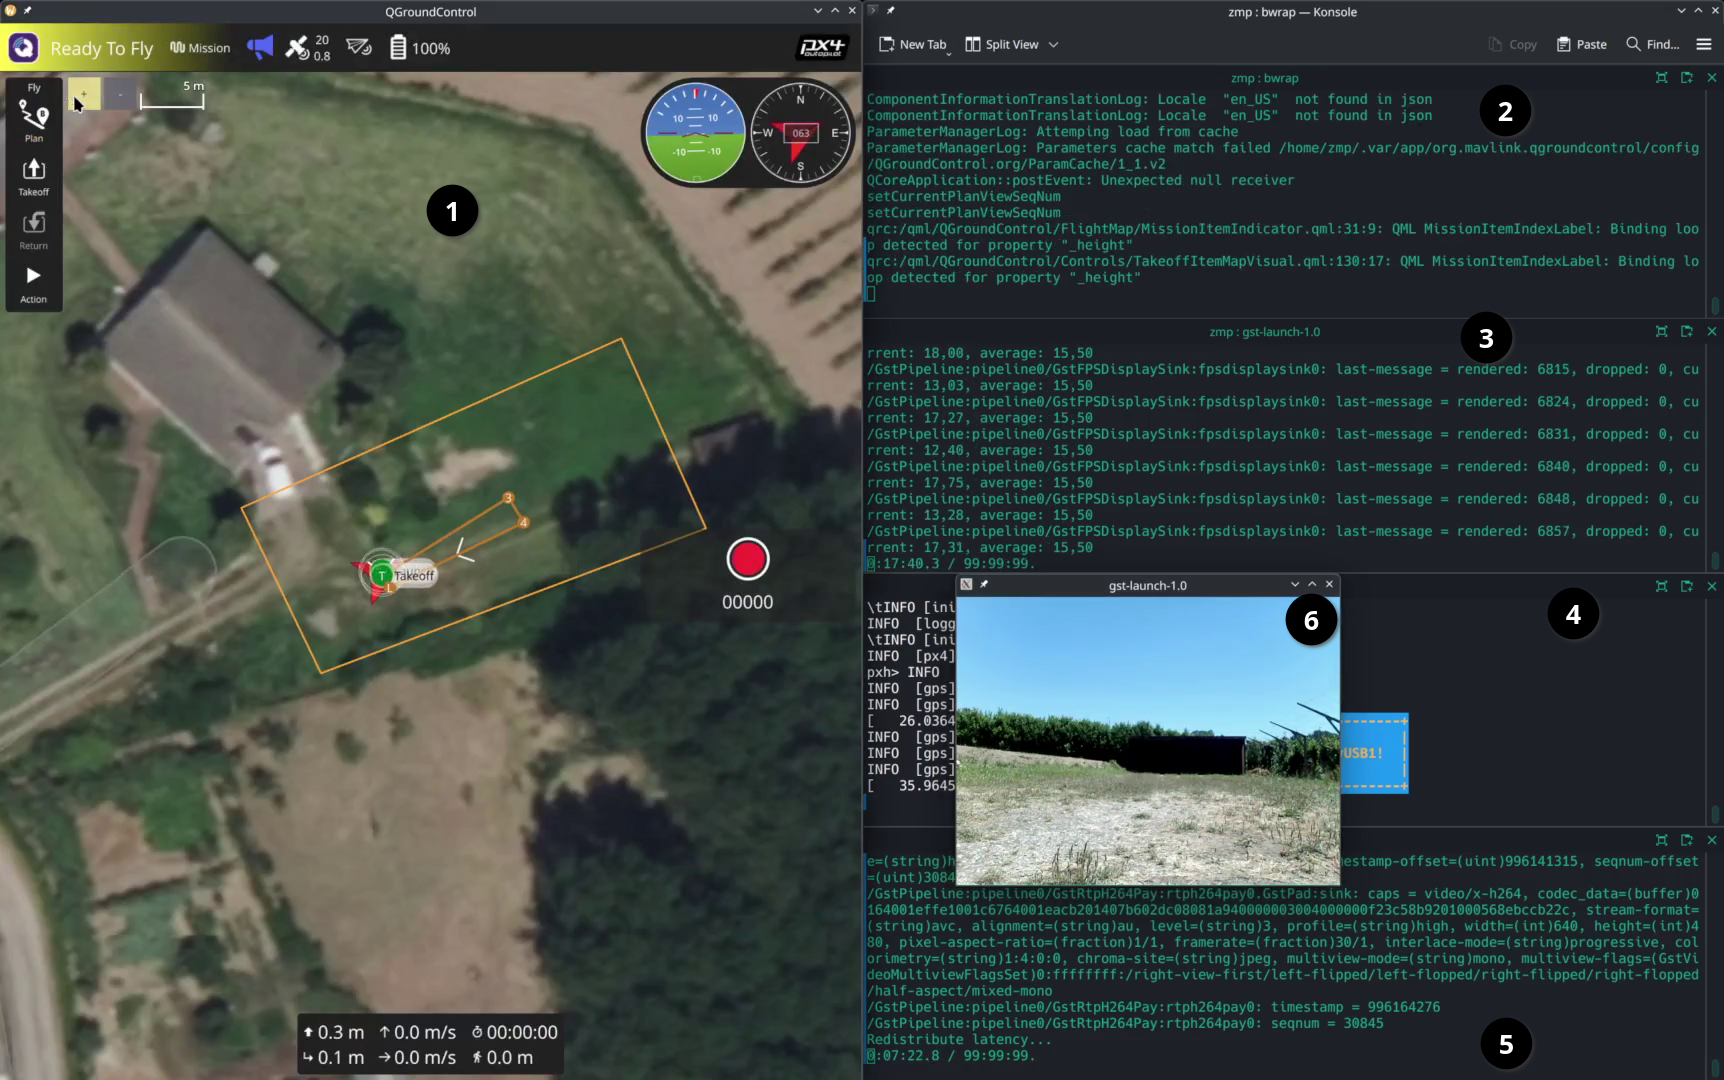
\includegraphics[width=1.0\textwidth]{./img/png/bao-fpv-takeoff-annot} 
    \caption{Takeoff}%
    \label{fig:mission-exec-case1}
  \end{subfigure}

  % Row 2: Two half-width images
  \begin{subfigure}[t]{0.49\textwidth}
    \centering
    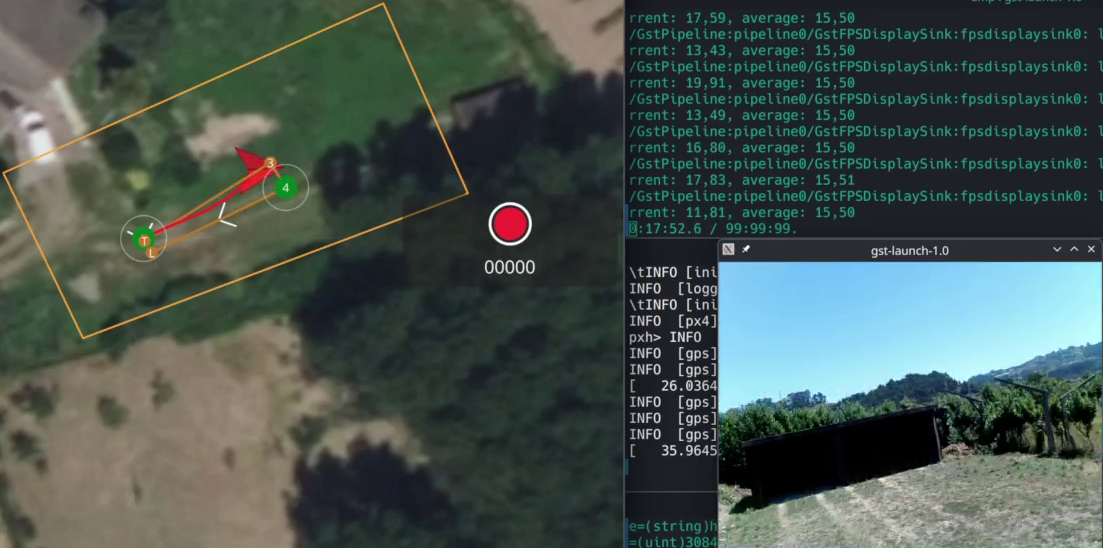
\includegraphics[width=\linewidth]{./img/png/bao-fpv-3-annot}
    \caption{Point 3}%
    \label{fig:mission-exec-case2}
  \end{subfigure}
  \hfill
  \begin{subfigure}[t]{0.49\textwidth}
    \centering
    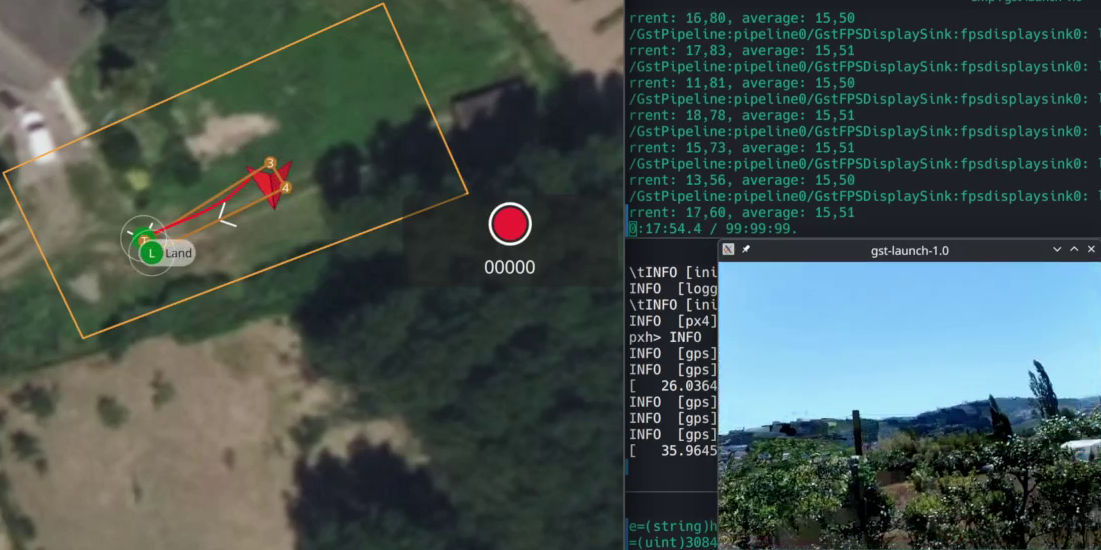
\includegraphics[width=\linewidth]{./img/png/bao-fpv-4-annot} 
    \caption{Point 4}%
    \label{fig:mission-exec-case3}
  \end{subfigure}

  % Row 3: Two half-width images
  \begin{subfigure}[t]{0.49\textwidth}
    \centering
    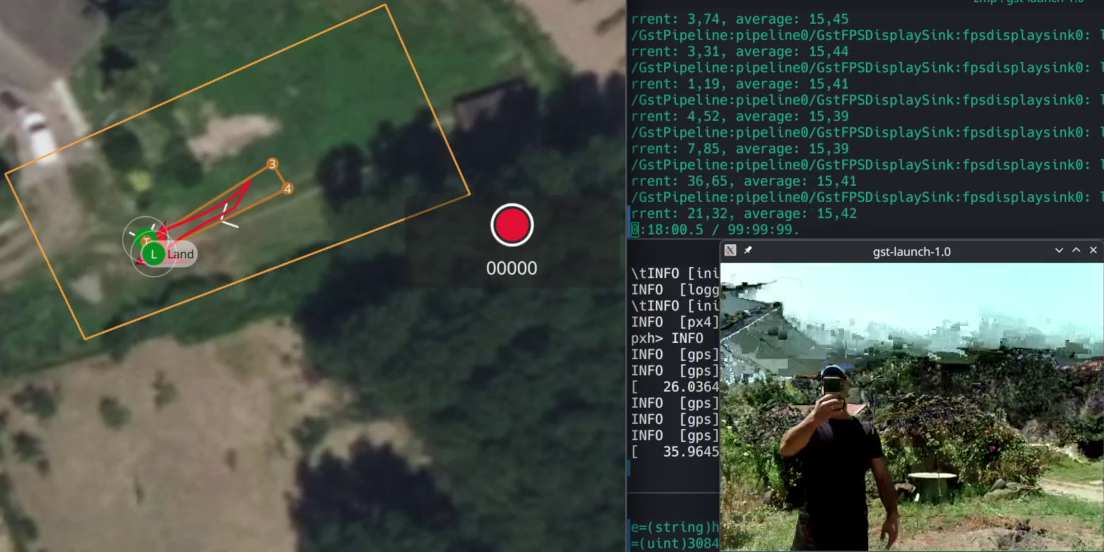
\includegraphics[width=\linewidth]{./img/png/bao-fpv-land-annot} 
    \caption{Landing}%
    \label{fig:mission-exec-case4}
  \end{subfigure}
  \hfill
  \begin{subfigure}[t]{0.49\textwidth}
    \centering
    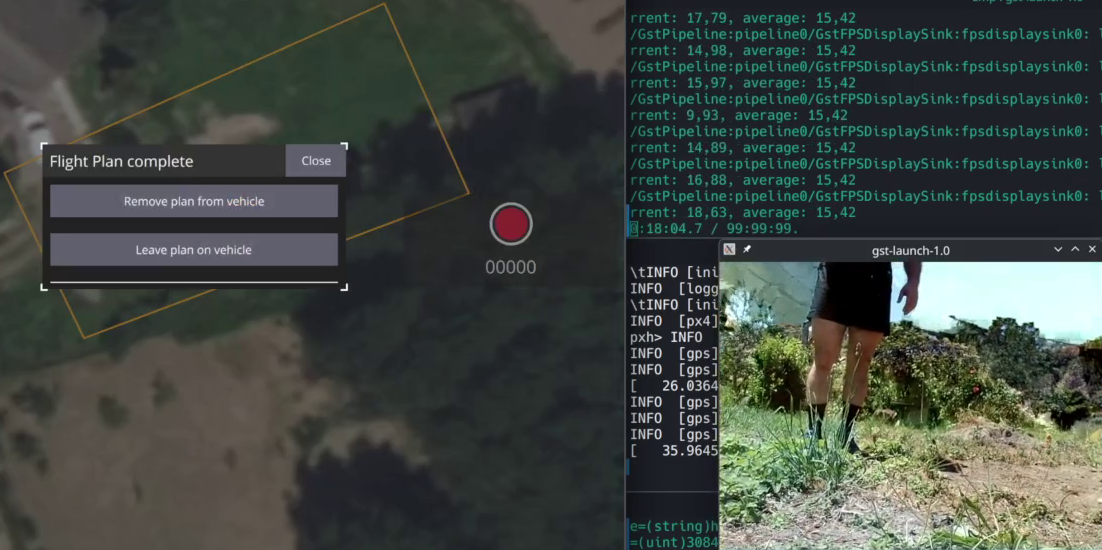
\includegraphics[width=\linewidth]{./img/png/bao-fpv-complete-annot} 
    \caption{Complete}%
    \label{fig:mission-exec-case5}
  \end{subfigure}
  
  \caption{Mission execution — SSPFS case}
  \label{fig:mission-exec-sspfs}
\end{figure}

Fig.~\ref{fig:mission-exec-case2} and Fig.~\ref{fig:mission-exec-case3}
show the flight path progression through the intermediate waypoints and the
corresponding video streaming.
Fig.~\ref{fig:mission-exec-case4} demonstrates the landing stage, showing the
\gls{uav} operator, and shortly after the mission is completed successfully
(Fig.~\ref{fig:mission-exec-case5}).
%
These results confirm that the \gls{sspfs} system functions as designed: the
autopilot operates within the \gls{fmu} \gls{vm}, exchanging data with the
\gls{gcs} through the telemetry radio link, while video streaming executes on
the \lstinline{Companion} \gls{vm}, capturing live feed from the \gls{usb} camera and transmitting it over Wi-Fi.

To interpret the test results we analyze the actual mission flight path,
illustrated as a red line in Fig.~\ref{fig:mission-final-actual}.
Mission paths exhibit slight variations due to differing sensor estimates and
weather conditions.
%
As anticipated, the autopilot dynamically adjusts trajectories according to
vehicle flight dynamics and parameters rather than strictly following predefined
paths. This adaptation is particularly evident during the sharp turn between
points \lstinline{3} and \lstinline{4}.
%
Consequently, although PX4 tries to adapt the trajectory to follow smooth
curves (defined by the acceptance radius parameter
\lstinline{NAV_ACC_RAD}~\cite{px4MissionModePath}), the velocity modulation
during approach and departure phases may limit this, based on jerk-limiting tuning parameters.

\begin{figure}[!hbt]
  \centering
  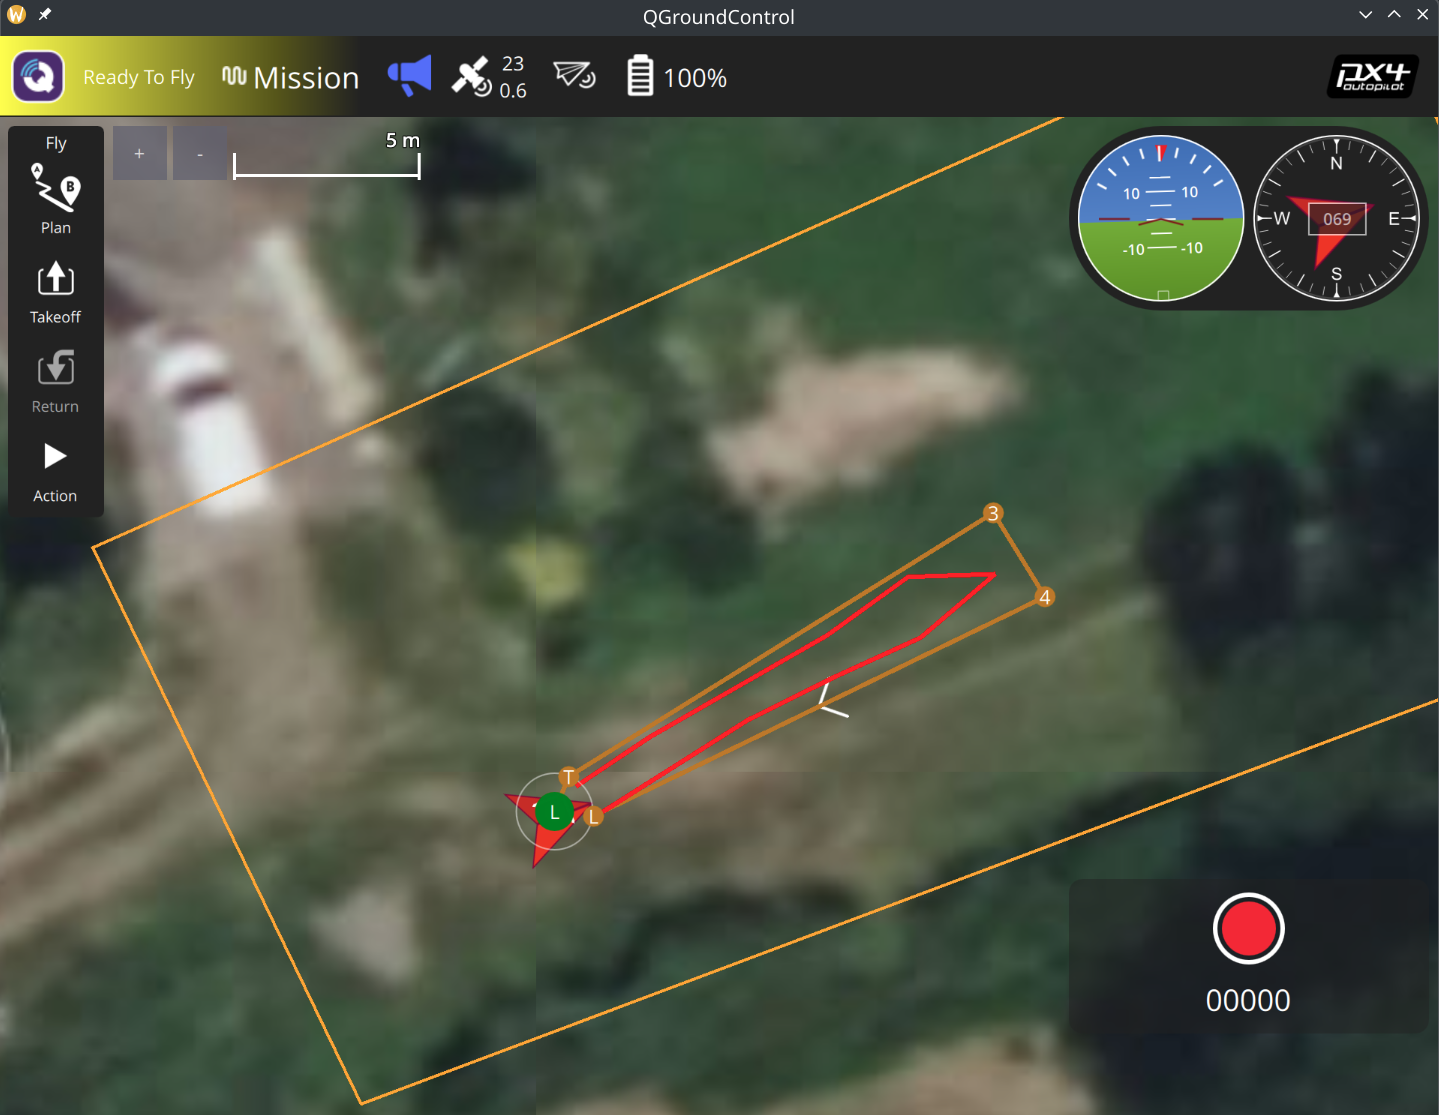
\includegraphics[width=0.8\textwidth]{./img/png/mission-final-actual} 
  \caption{Actual flight path of a mission in QGroundControl}%
  \label{fig:mission-final-actual}
\end{figure}

Fig.~\ref{fig:pos-track-cmp} presents the comparison in position 
tracking performance between the \gls{uspfs} and \gls{sspfs}
systems across X, Y, and Z axes.
%
The solid lines indicate the actual trajectories, while the dotted ones
represent the setpoint trajectories. The blue and orange traces correspond to
the \gls{uspfs} and \gls{sspfs} systems, respectively, with the shaded
bands denoting the 95\% confidence intervals for the mean.
%
The controller demonstrates accurate position tracking, with the observed
trajectories closely following setpoints except during takeoff and landing
phases due to flight dynamics.
%
Notably, setpoint variations occur between systems despite identical
missions. This can be attributed to differing flight dynamics influenced by
environmental factors, particularly air pressure variations affecting Z-axis
estimates~\cite{px4-static-pressure,px4-static-pressure-correc}, and sensor
estimation discrepancies, such as noise in the \gls{gps} measurements.
%
The significant overlap between the actual and setpoint bands indicates no statistical difference in X and Z-axis
tracking between systems. However, a consistent Y-axis offset of approximately 2
meters is observed. Further data collection is needed to investigate the underlying causes of
this deviation. Nonetheless, adding supervision to the autopilot shows no adverse impact on overall position tracking performance.

\begin{figure}[!hbt]
  \centering
  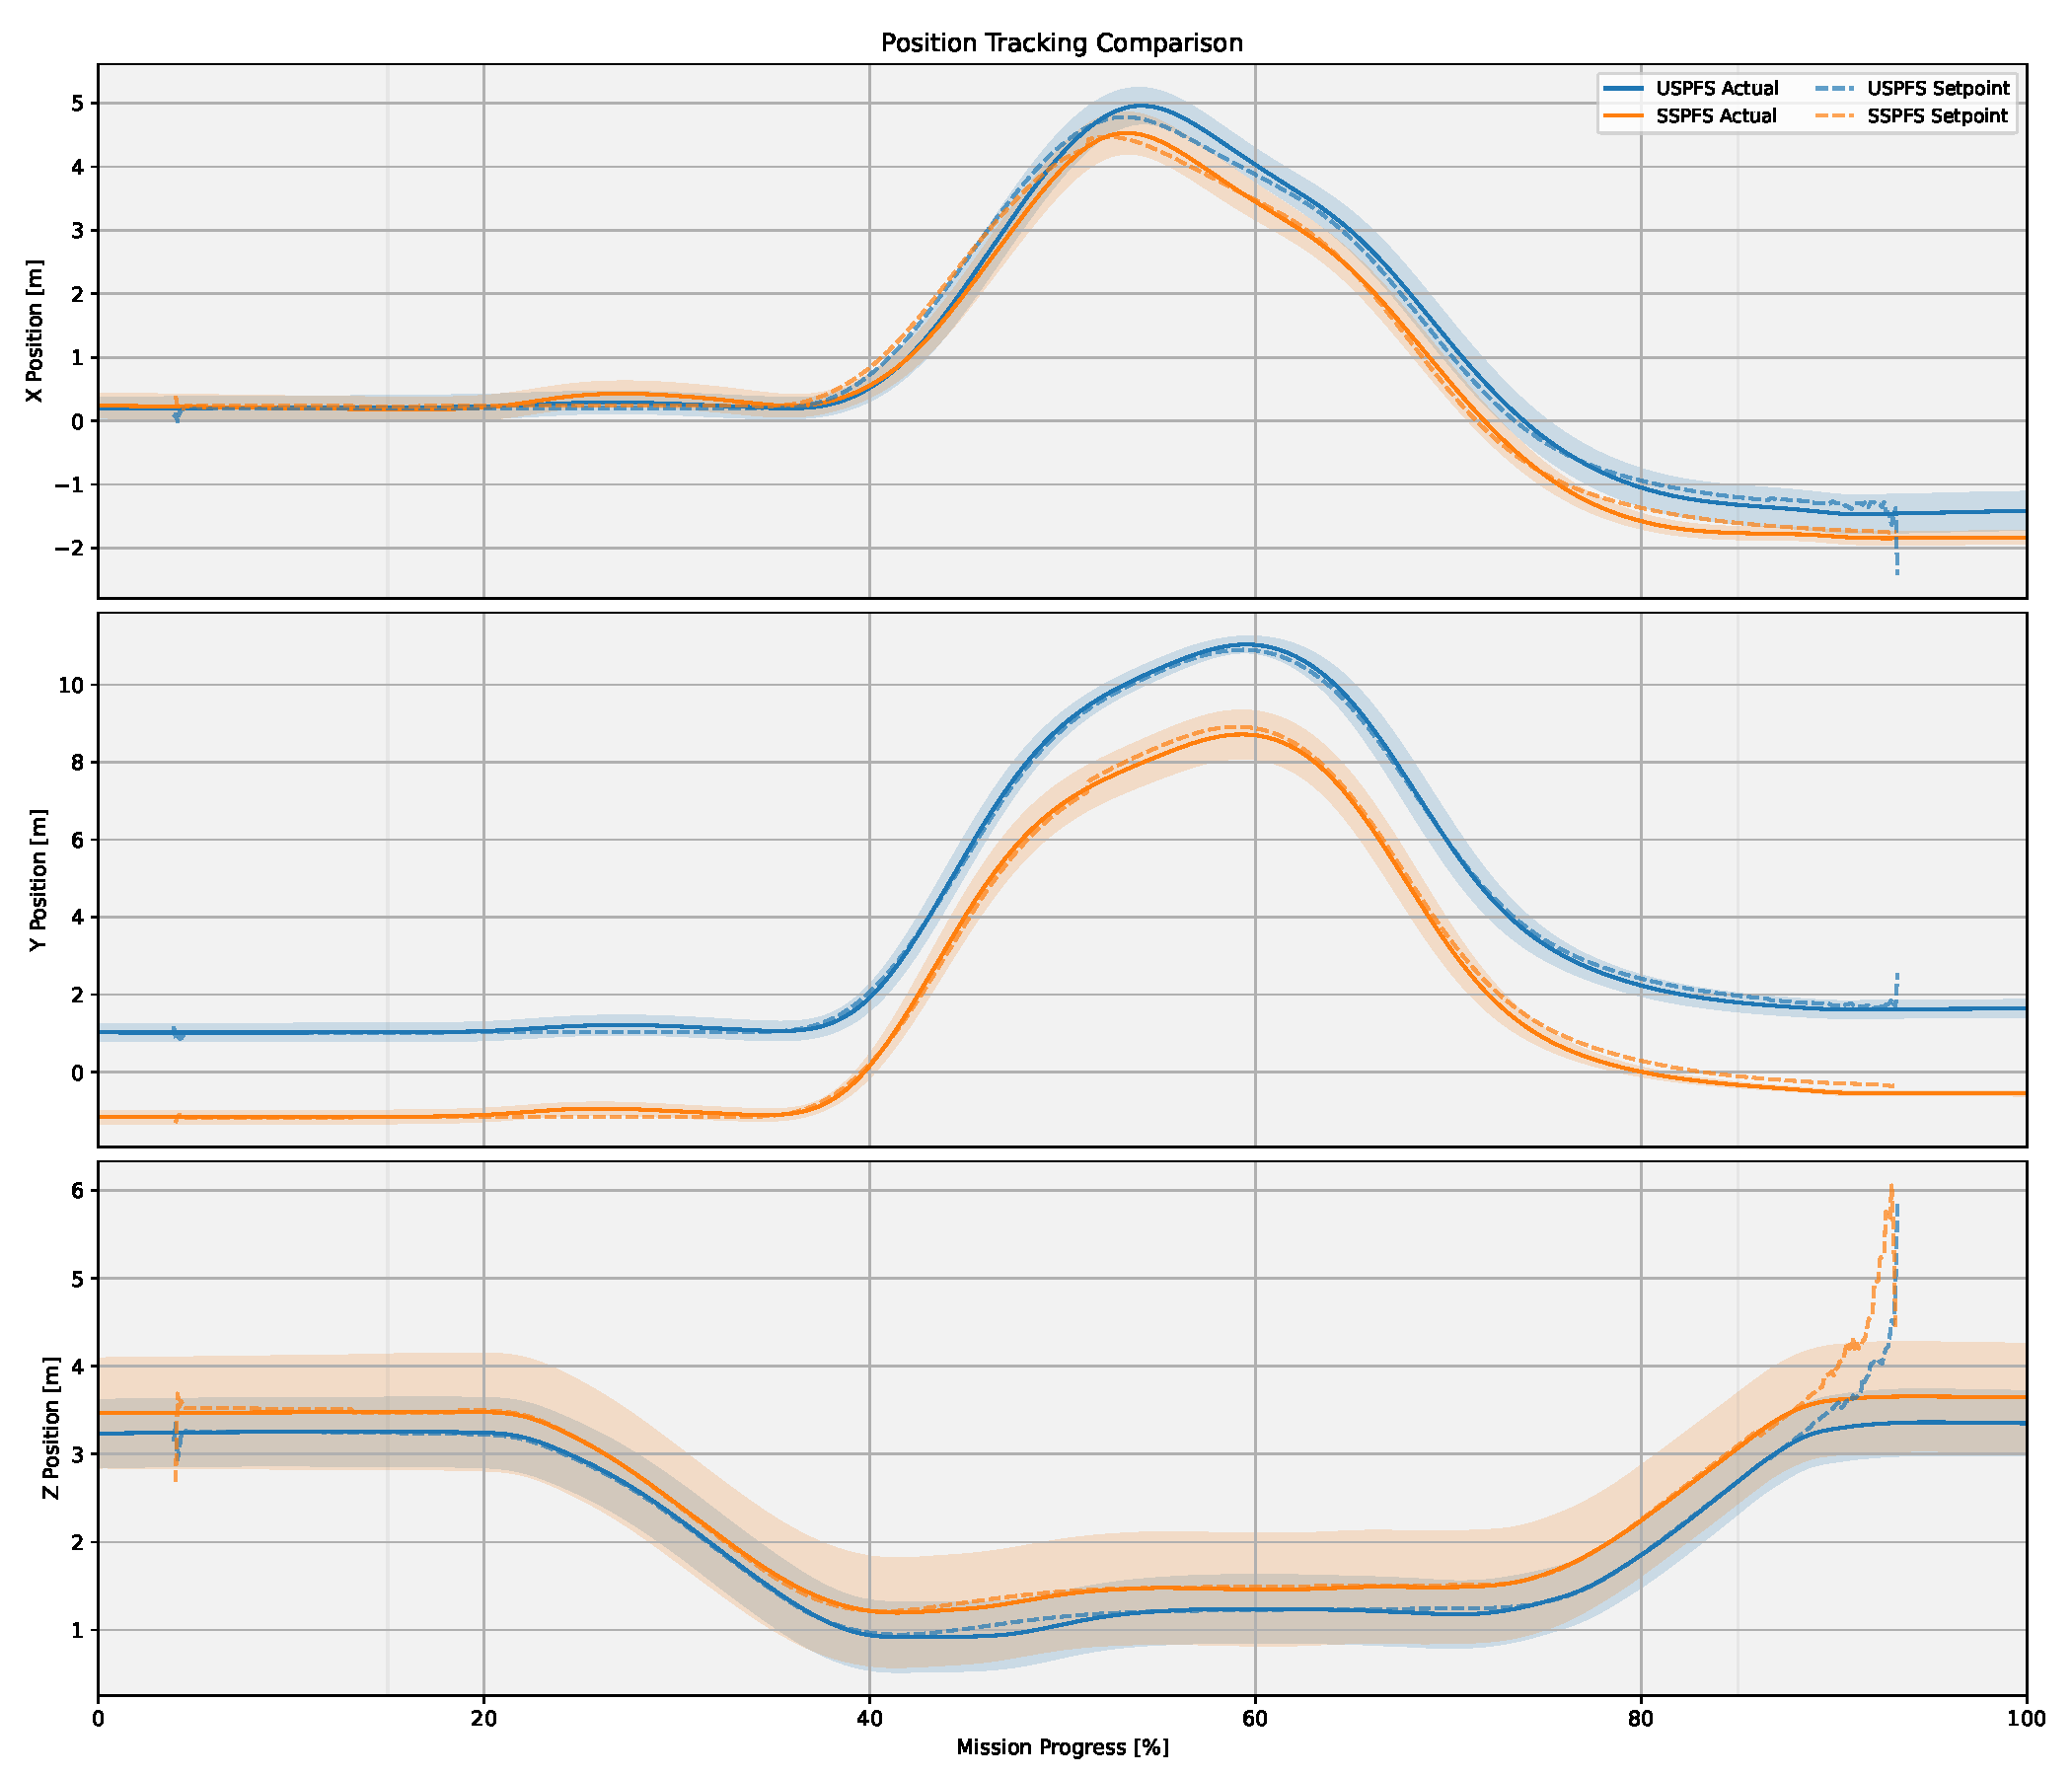
\includegraphics[width=1.0\textwidth]{./img/pdf/pos-track-cmp} 
  \caption{Position tracking comparison between USPFS and SSPFS systems}%
  \label{fig:pos-track-cmp}
\end{figure}

We compared resource usage between the \gls{uspfs} and \gls{sspfs} using
PX4 \gls{uorb}-derived proxies rather than direct host-side measurements
(Fig.~\ref{fig:sys-resources-cmp}). The supervised system shows an
\(\approx 6\%\) increase in \gls{cpu} load and about a ninefold rise in
PX4-reported \gls{ram} use. The \gls{cpu} delta is consistent with prior Bao
results (Section~\ref{sec:bao-benchmarks}). The \gls{ram} increase is best
explained as the combination of \emph{SSPFS baseline costs} (per-guest
stage-2 page tables and small Bao metadata/state) and \emph{mailbox-related
driver allocations} in Linux (transient request/response buffers and slab
caching), rather than the mailbox supervisor alone. No hypervisor-managed
shared-memory window is introduced by our design. In absolute terms, the
increase is small relative to the \gls{fmu} \gls{vm}'s 144\,MB budget
(about 90\,kB in \gls{sspfs} versus 10\,kB in \gls{uspfs}). Because these
metrics are indirect, host-side accounting would be required to analyze
overhead more precisely.

\begin{figure}[!hbt]
  \centering
  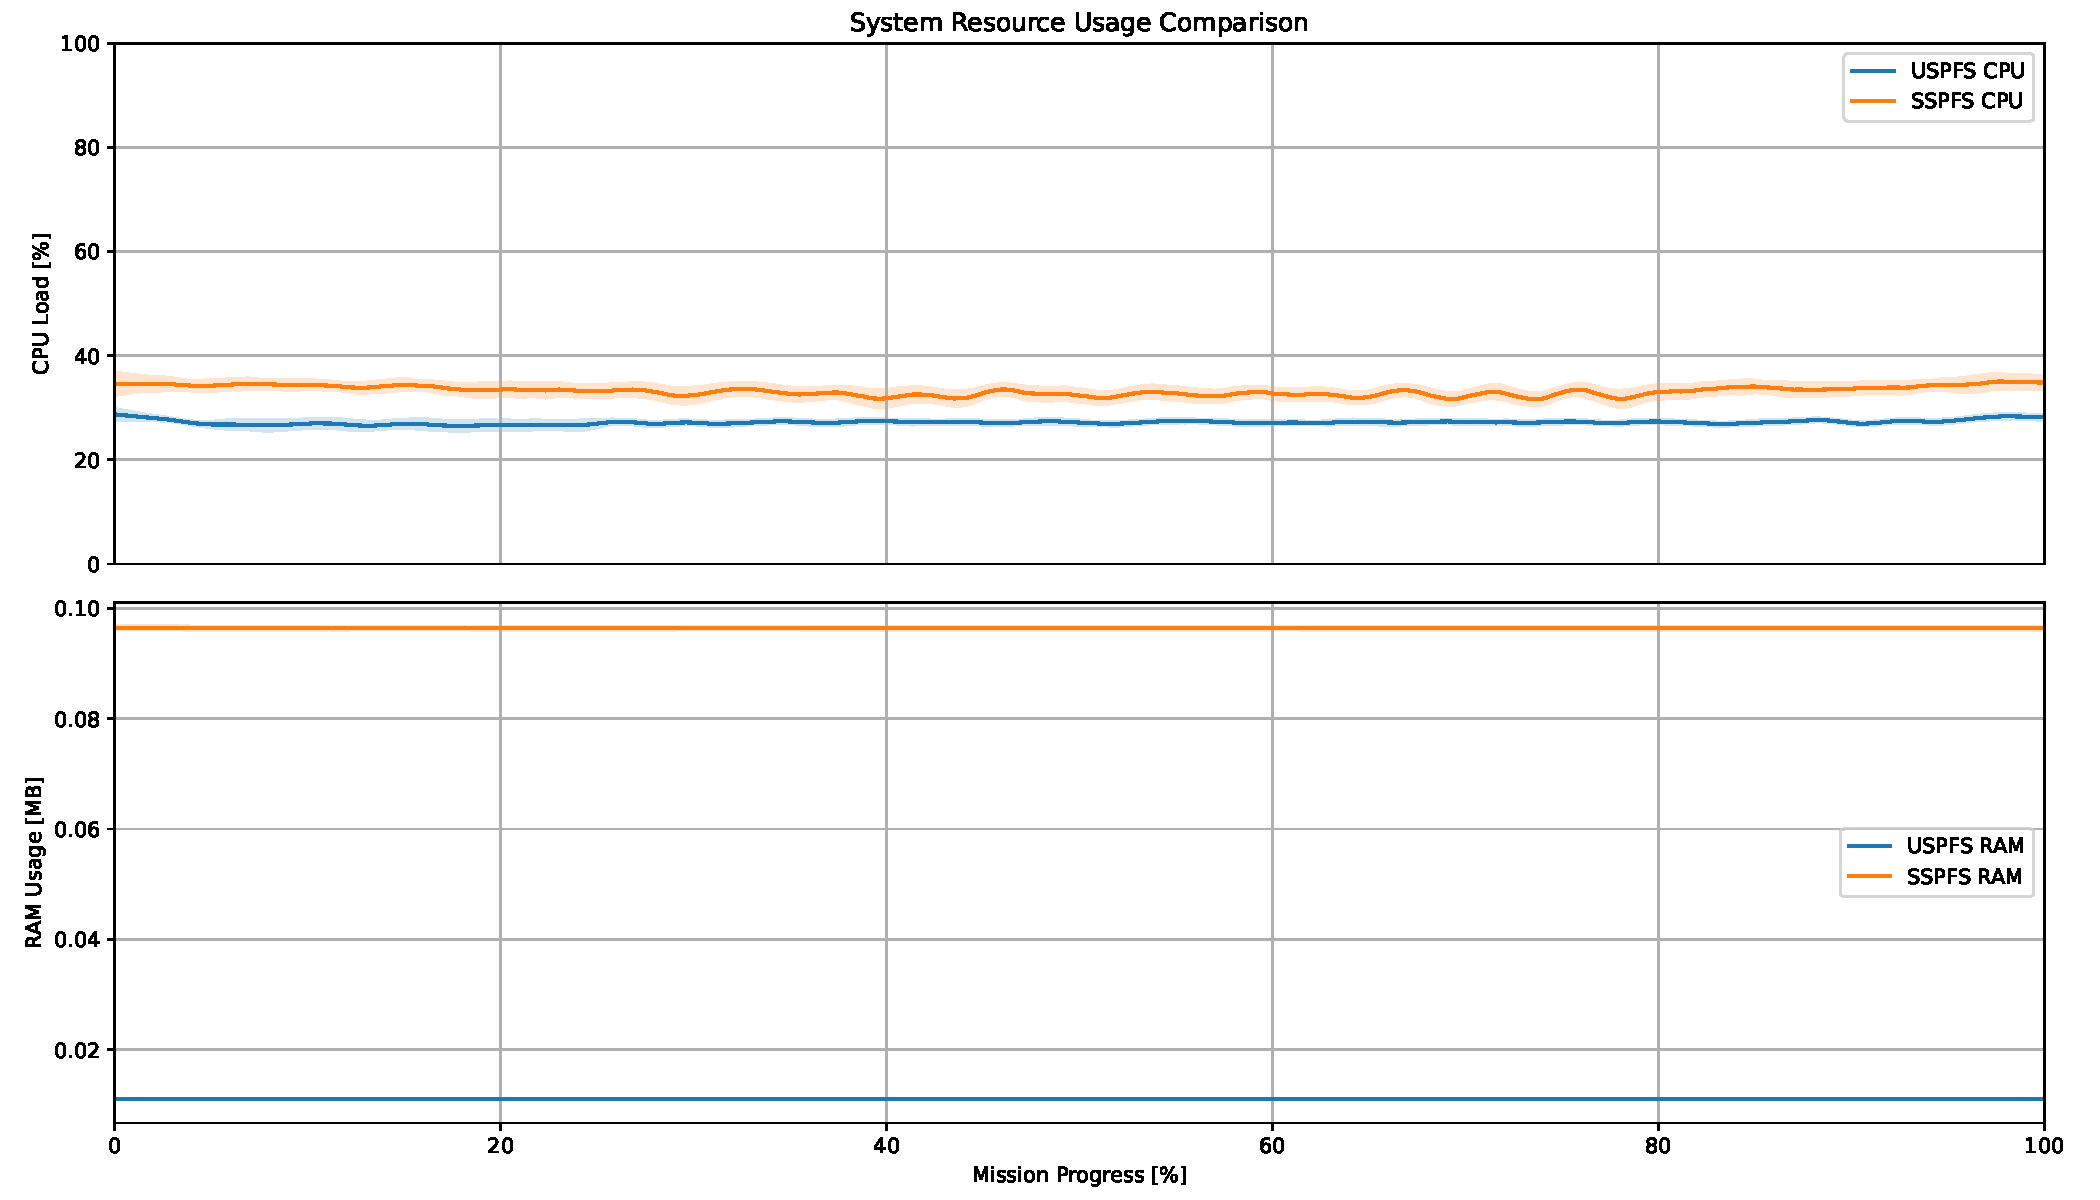
\includegraphics[width=1.0\textwidth]{./img/pdf/sys-resources-cmp} 
  \caption{System resource usage comparison between USPFS and SSPFS systems}%
  \label{fig:sys-resources-cmp}
\end{figure}

The functional tests were replicated in real-flight scenarios. They are fully
detailed in videos available in the online repository~\cite{thesis-sw-github}.
Fig.~\ref{fig:mission-exec-sspfs-last} demonstrates the \gls{sspfs} system behavior
during a system compromise. Fig.~\ref{fig:mission-exec-sspfs-takeoff-1} shows
the software tools used and the \gls{uav}'s flight view: (1) QGroundControl
mission planning and tracking; (2) \lstinline{gstreamer} receiver pipeline
running at the \gls{gcs} and its \gls{gui} (6); telemetry data collected by PX4
and accessible through QGroundControl (3); (4) U-Boot loader and
\gls{fmu} \gls{vm} executing PX4; (5) \lstinline{Companion}
\gls{vm} running the \lstinline{gstreamer} sender pipeline and accessible via
\gls{ssh} over Wi-Fi; (7) and a remote \gls{ssh} shell to compromise the Companion
\gls{vm}. We observe that the video streaming is operating normally during
takeoff and that the \gls{uav} starts to fly (Fig.~\ref{fig:mission-exec-sspfs-takeoff-2}).
We then executed the malicious kernel module within the \lstinline{Companion}
\gls{vm}. Video streaming immediately froze, indicating compromised
functionality in this \gls{vm}. Despite this failure, the \gls{uav} lands (Fig.~\ref{fig:mission-exec-sspfs-final}),
indicating that PX4 remained fully operational and, thus, the mission completed successfully.
%
These results demonstrate Bao's hypervisor capability to effectively isolate the
critical flight stack (\gls{fmu} \gls{vm}) from non-critical components
(\lstinline{Companion} \gls{vm}).
Consequently, crashes in the \lstinline{Companion} \gls{vm} remain contained without propagating to the autopilot, preventing potential catastrophic \gls{uav} failure.

\begin{figure}[!hbt]
  \centering
  % Row 1: Full width
  \begin{subfigure}[t]{\textwidth}
    \centering
    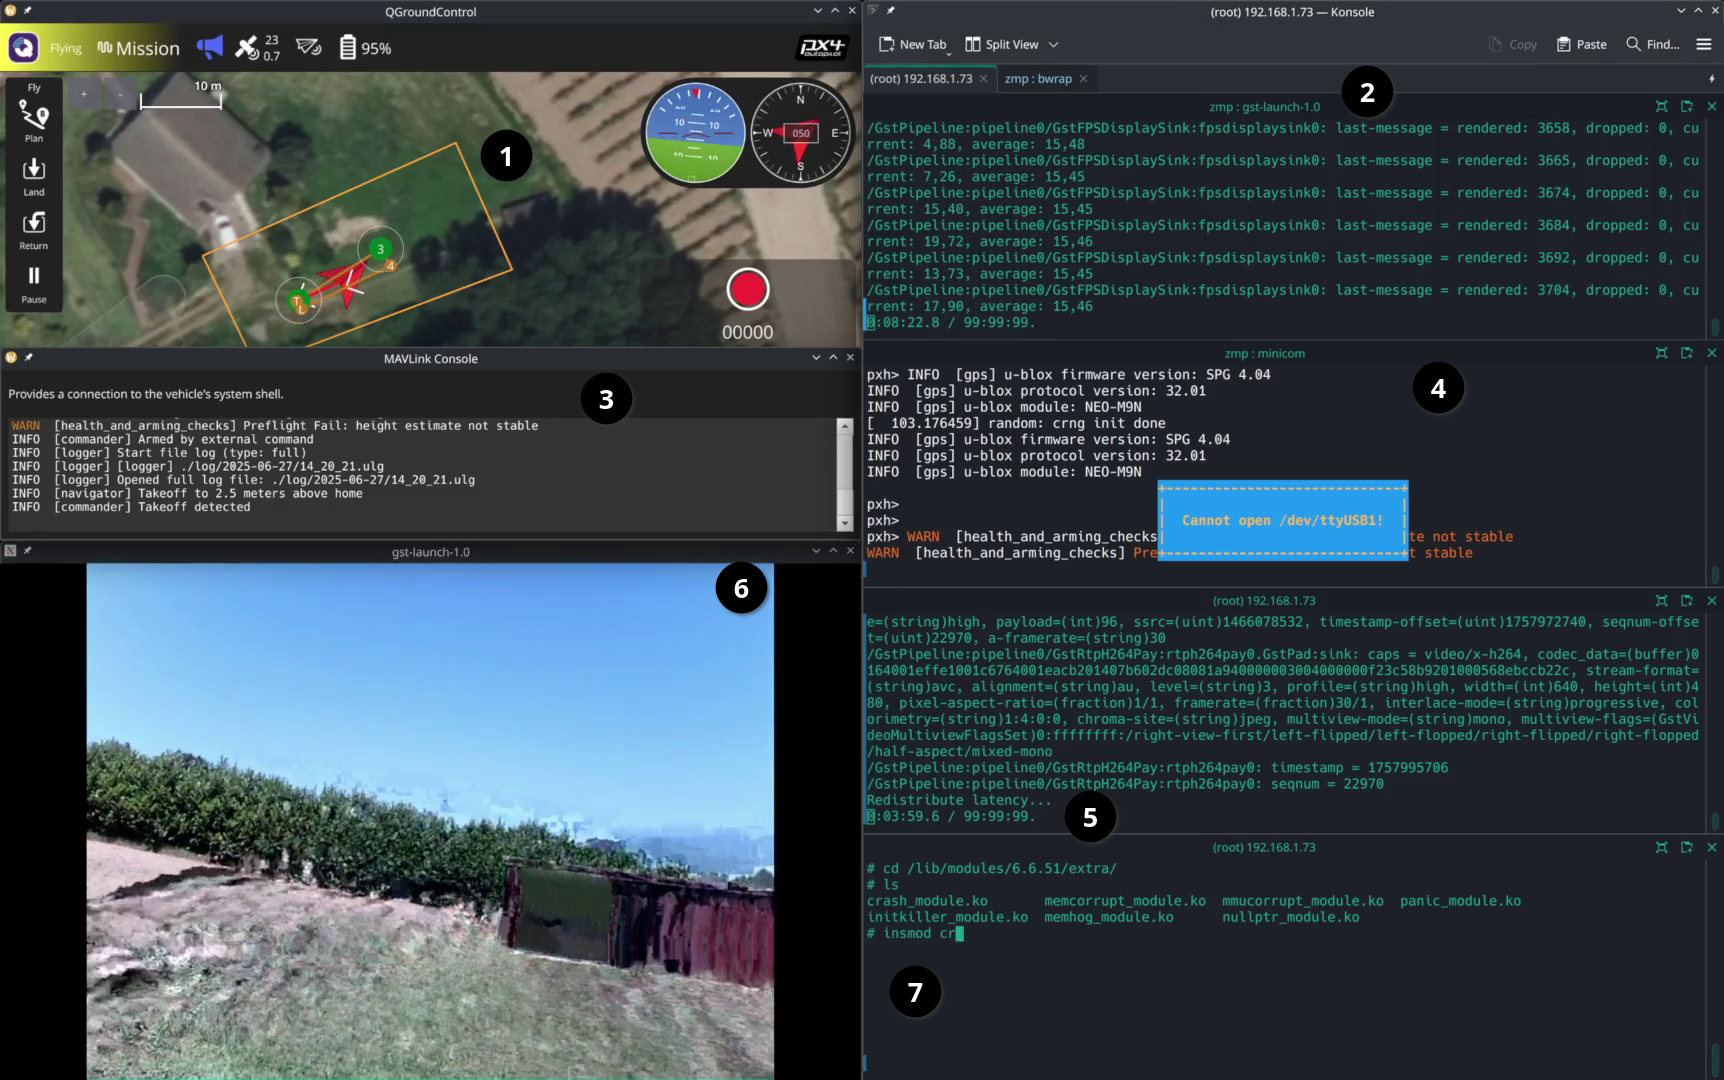
\includegraphics[width=1.0\textwidth]{./img/png/bao-fpv-insmod-1} 
    \caption{UAV's view: takeoff}%
    \label{fig:mission-exec-sspfs-takeoff-1}
  \end{subfigure}
%  
  % Row 2: Two half-width images
  \begin{subfigure}[t]{0.49\textwidth}
    \centering
    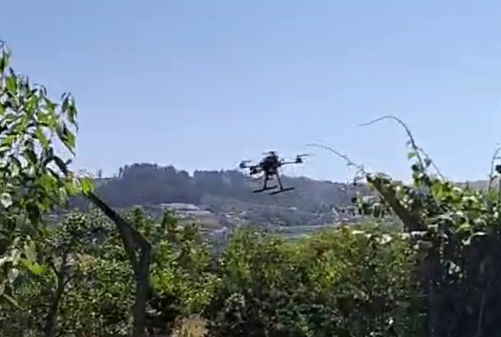
\includegraphics[width=\linewidth]{./img/png/bao-flight-myView-takeoff}
    \caption{Operator's view: takeoff}%
    \label{fig:mission-exec-sspfs-takeoff-2}
  \end{subfigure}
  \begin{subfigure}[t]{0.49\textwidth}
    \centering
    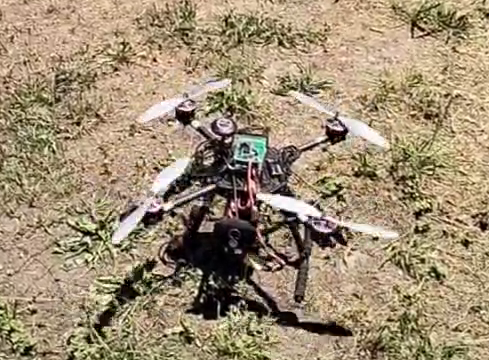
\includegraphics[width=0.92\linewidth]{./img/png/bao-flight-myView-final}
    \caption{Operator's view: successful landing}%
    \label{fig:mission-exec-sspfs-final}
  \end{subfigure}
%  
  \caption{Mission execution: functional test (SSPFS)}
  \label{fig:mission-exec-sspfs-last}
\end{figure}

The same functional test procedure was subsequently applied to the \gls{uspfs}
system.
Fig.~\ref{fig:mission-exec-uspfs} demonstrates the \gls{uspfs} system behavior
during a system compromise. Fig.~\ref{fig:mission-exec-uspfs-takeoff-1} shows
the software tools used and the \gls{uav}'s flight view: (1) QGroundControl
mission planning and tracking, and logs (2); (3) \lstinline{gstreamer} receiver pipeline
running at the \gls{gcs} and its \gls{gui} (4); telemetry data collected by PX4
and accessible through QGroundControl (3); (6) PX4 application running in the
\gls{uspfs}; (5) \lstinline{gstreamer} sender pipeline
running on the \gls{uspfs} and accessible via
\gls{ssh} over Wi-Fi; (7) a remote \gls{ssh} shell to compromise the
\gls{uspfs} system. We observe that video streaming operates normally during
takeoff and that the \gls{uav} starts to fly (Fig.~\ref{fig:mission-exec-uspfs-takeoff-2}).
We then executed the malicious kernel module within the \gls{uspfs}
system. Video streaming immediately froze, indicating system failure,
and the \gls{uav} began erratic maneuvers until it crashed
(Fig.~\ref{fig:mission-exec-uspfs-final}).
%
This outcome demonstrates that in unsupervised architectures, non-critical
component failures propagate system-wide, resulting in catastrophic \gls{uav}
loss.

\begin{figure}[!hbt]
  \centering
  % Row 1: Full width
  \begin{subfigure}[t]{\textwidth}
    \centering
    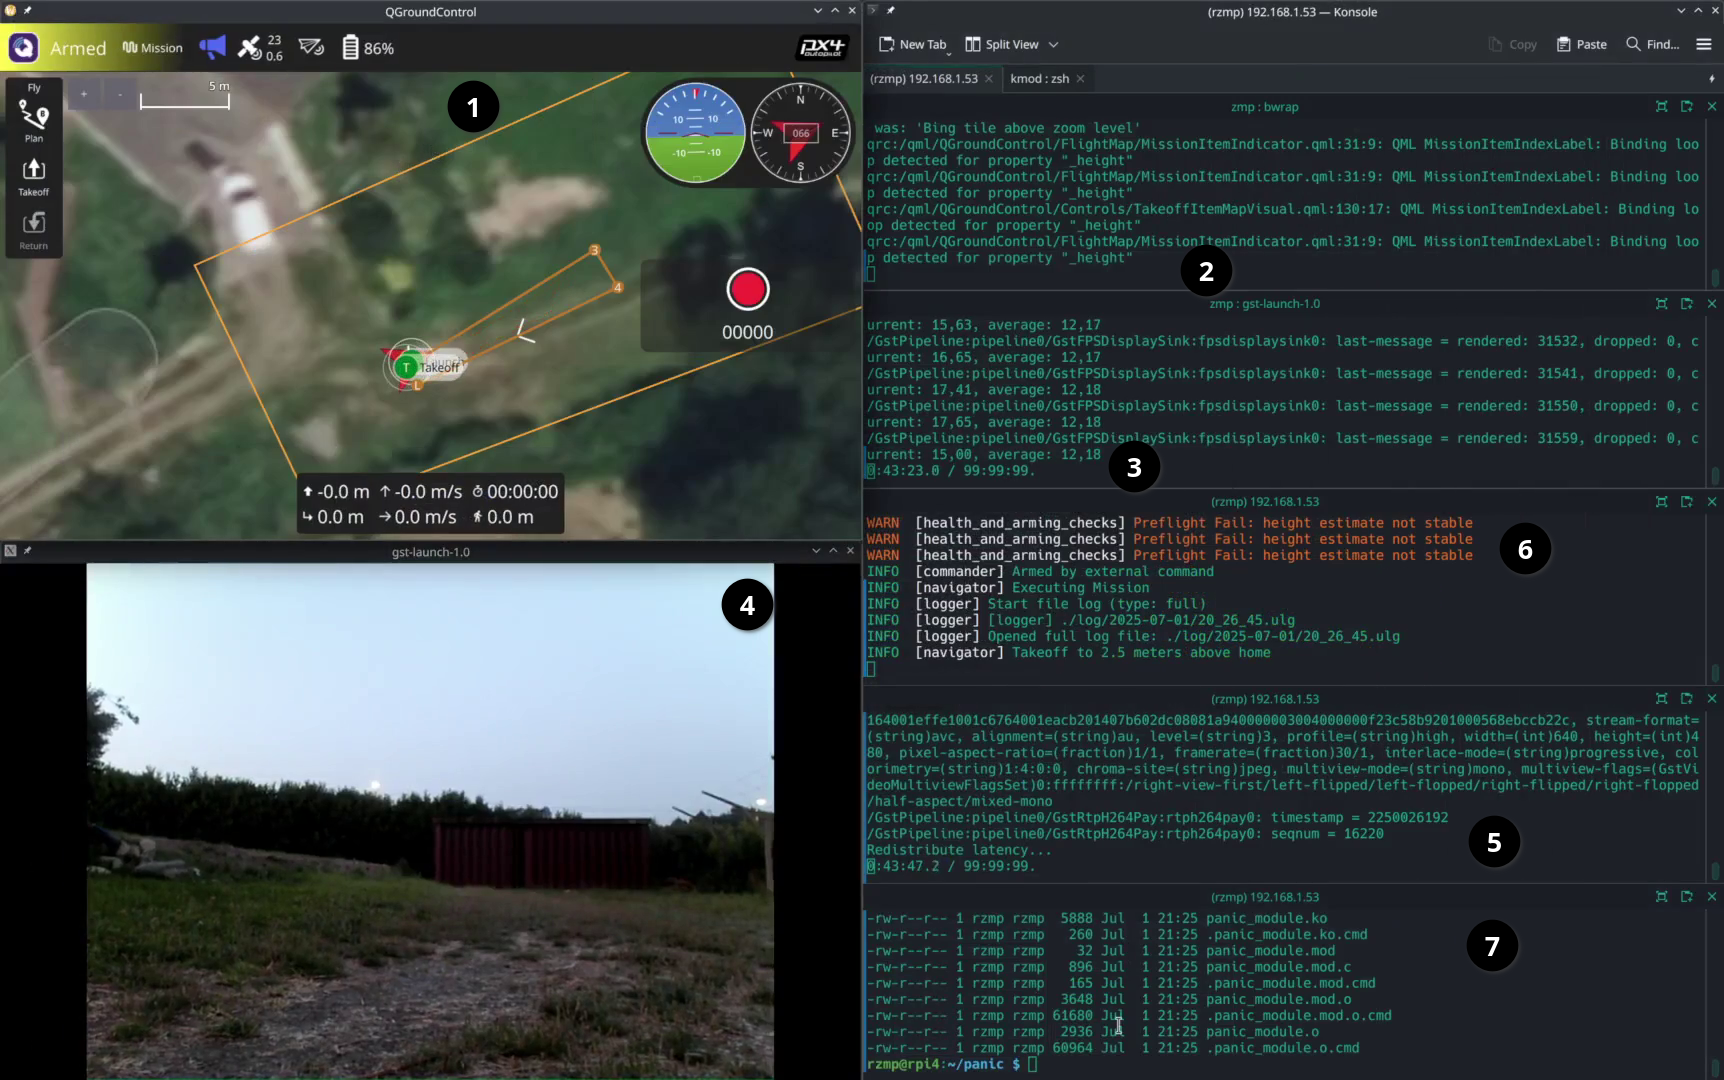
\includegraphics[width=1.0\textwidth]{./img/png/uspfs-crash-fpv-takeoff-annot} 
    \caption{UAV's view: takeoff}%
    \label{fig:mission-exec-uspfs-takeoff-1}
  \end{subfigure}
%  
  % Row 2: Two half-width images
  \begin{subfigure}[t]{0.49\textwidth}
    \centering
    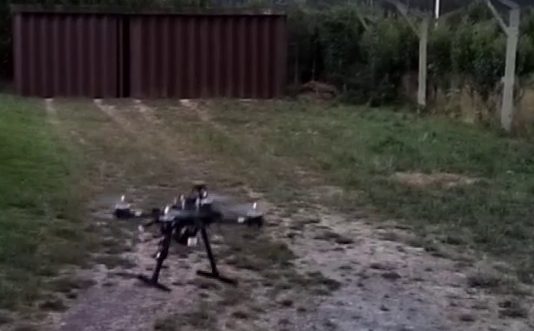
\includegraphics[width=0.98\linewidth]{./img/png/uspfs-crash-myView-takeoff-crop}
    \caption{Operator's view: takeoff}%
    \label{fig:mission-exec-uspfs-takeoff-2}
  \end{subfigure}
  \begin{subfigure}[t]{0.49\textwidth}
    \centering
    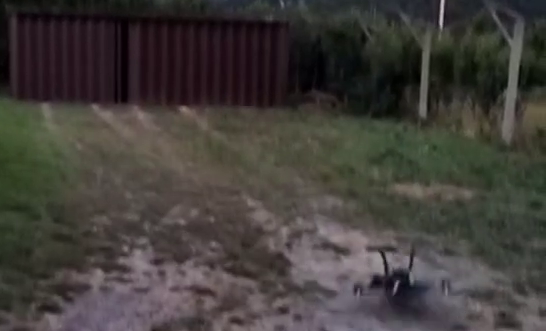
\includegraphics[width=\linewidth]{./img/png/uspfs-crash-myView-final-crop}
    \caption{Operator's view: UAV crash}%
    \label{fig:mission-exec-uspfs-final}
  \end{subfigure}
%  
  \caption{Mission execution: functional test (USPFS)}
  \label{fig:mission-exec-uspfs}
\end{figure}

%%% Local Variables:
%%% mode: latex
%%% TeX-master: "../template"
%%% reftex-default-bibliography: ("../Bibliography/mieeic.bib")
%%% ispell-local-dictionary: "american"
%%% End:
